\graphicspath{{chapter1/}{manuscript/}}

\chapter{\textbf{\MakeUppercase{  L'aménagement forestier pourrait
accélérer le déplacement des arbres tempérés face au changement
climatique}}}

\section{Résumé de l'article et contribution}

De nombreuses espèces d'arbres assciées à une démographie lente, une
dispersion limitée et une forte compétition devraientt présenter un
retard de migration vers le nord en comparaison à l'évolution des
changements climatiques. Cela se traduira par un crédit de colonisation,
lorsque les enveloppes climatiques appropriées resteront inoccupées, et
par une dette d'extinction, lorsque les peuplements d'arbres
persisteront dans des enveloppes climatiques inappropriés. Bien que les
mécanismes sous-jacents expliquant le changement tardif de l'aire de
répartition des arbres forestiers soient bien étudiés, peu d'études se
sont concentrées sur le potentiel de l'emménagement forestier pour
surmonter ce décalage.\\

Dans ce chapitre, nous avons développé un modèle d'état des communautés
forestières dérivé de la théorie des métapopulations et testé avec plus
de 40 000 parcelles d'inventaire forestier afin de comprendre comment
l'emménagent forestier pourrait accélérer la réponse de l'écotone
boréal-tempéré au réchauffement des températures. Dans un premier temps,
nous avons complété les équations du modèle pour étudier comment quatre
pratiques d'emménagement peuvent affecter les transitions entre quatre
états forestiers~: Boréal, Tempéré, Mixte et Régénération. Dans un
second temps, nous avons simulé le potentiel de l'emménagement forestier
pour réduire le crédit de colonisation et la dette d'extinction en
utilisant deux approches complémentaires. La première méthode mesure la
résilience des forêts basée sur la dynamique transitoires alors que la
deuxième méthode mesure le déplacement de l'écotone boréal-tempéré dans
une gride spatiale en réponse au réchauffement de la température.\\

Nos simulations ont révélé que payer le crédit de colonisation en
plantant des arbres tempérés dans un peuplement en Régénération ou en
état Boréal est susceptible de i) réduire le temps de retour à
l'équilibre, ii) augmenter la résilience des forêts et iii) déplacer
l'écotone vers des températures plus froides. Étonnamment, la récolte
d'arbres boréaux dans des peuplements boréaux ou mixtes n'a pas été
efficace pour réduire la dette d'extinction.\\

Deplus, l'exploitation des arbres boréaux dans des peuplements en état
Boréal ou Mixte n'était pas efficace pour réduire la dette d'extinction
et offrir des opportunités de colonisation pour les arbres tempérés. Nos
résultats suggèrent que l'emménagement forestier liée aux actions de
plantation pourrait aider l'écotone boréal-tempéré à suivre le rythme du
changement climatique. De futures expérimentations sont nécessaires pour
tester ces attentes théoriques et formuler des recommandations
opérationnelles.\\

Cette étude a été conçu par Dominique Gravel et moi-même. Le
développement du modèle et les analyses ont été produits par Isabelle
Boulangeat et moi-même. Les figures et la rédaction de la première
version du manuscrit ont été effectuées par moi-même. Toutes les
co-auteur.e.s ont contribué aux revisions du manuscrit. Cet article est
présentement en révision dans la revue \emph{Ecological Modelling}.\\

\vfill{}
\pagebreak

\begin{center}
\textbf{\MakeUppercase{Paying colonization credit with forest management
could accelerate the range shift of temperate trees under climate
change}} \\
Willian~Vieira, Isabelle~Boulangeat, Marie-Hélène~Brice, Robert
L.~Bradley, Dominique~Gravel
\end{center}

\section{Abstract}

The northward migration of several tree species ranges is likely to lag
behind climate change due to slow demography, competitive interactions,
and dispersal limitations. These will result in a colonization credit,
where suitable climate envelopes are left unoccupied, and extinction
debt, where tree stands persist at unsuitable climatic locations. While
the underlying mechanisms explaining the delayed range shift of forest
trees have been investigated, few studies have focused on how management
could overcome this lag. Here we extend a forest community state model
derived from the metapopulation theory and validated with over 40,000
forest inventory plots, to formulate how forest management can
accelerate the response of the boreal-temperate ecotone under warming
temperature. We first complete the model equations to represent how four
types of forest management may affect the transitions between four
forest states: Boreal, Temperate, Mixed and Regeneration. We then
simulated the potential of forest management to reduce colonization
credit and extinction debt using two complementary approaches to measure
the resilience and range shift of the boreal-temperate ecotone in
response to warming temperature. Our simulations reveal that paying the
colonization credit by planting temperate trees in a stand in
Regeneration or Boreal state are likely to i) reduce the return time to
equilibrium, ii) increase forest resilience, and iii) move the ecotone
towards colder temperatures. Surprisingly, harvesting boreal trees in
stands in Boreal or Mixed state were not effective to reduce extinction
debt and provide colonization opportunities for temperate trees. Our
results suggest that forest management related to planting actions could
help the boreal-temperate ecotone keep pace with climate change. Future
experiments are required to test these theoretical expectations and make
operational recommendations.\\

\textbf{Keywords}: Adaptive management, Assisted
migration, Resilience, Range dynamics, Transient
dynamics, Metapopulation, State and Transition Models

\hypertarget{introduction}{%
\section{Introduction}\label{introduction}}

There is a growing concern about how tree species will respond to
climate change, and how fast they can migrate to keep pace with climate
warming. Correlative statistical models have projected large range
shifts following temperature increases, such as the migration of plant
species hundreds of kilometers northward by the end of this century
\citep{Malcolm2002, Mckenney2007}. While the range of short-lived mobile
species may keep pace with climate change \citep{Chen2011}, the range of
long-lived tree species generally does not \citep{Harsch2009, Zhu2012}.
In fact, trees of eastern North America have shifted their range limits
way bellow of the pace required to keep up with temperature increases
\citep{BoisvertMarsh2014, BoisvertMarsh2019, Sittaro2017}. This mismatch
between climate conditions and forest community composition will likely
lead to maladaptation of trees to their environment, and therefore a
possible loss of future forest productivity \citep{Aitken2008}.
Assessing the mechanisms determining species range limits is, therefore,
critical for formulating adaptive management strategies
\citep{Becknell2015a}.\\

Range limits of forest trees are driven by colonization and extinction
dynamics. The metapopulation theory predicts the boundary of a species'
range occurs where the colonization rate equals the extinction rate,
wherever habitat is available \citep{Holt2000}. Derived from this
theory, \citet{Talluto2017} quantified the colonization and extinction
rates as a function of climate for 21 tree species in eastern North
America and found that their distribution is out of equilibrium with the
current climate. Specifically, they found a colonization credit at the
leading edge of their range whereby suitable habitat is left unoccupied,
and an extinction debt at the trailing edge whereby populations persist
in unsuitable habitats. This equilibrium mismatch is predicted to
increase in the future, as the range limits of temperate trees will
barely shift northward due to their slow demography and limited
dispersal rates \citep{Vissault2020}.\\

Forest management provides an opportunity to reduce colonization credit
and extinction debt and, therefore, accelerate range shifts. Although
some management practices, such as assisted migration
\citep{Peters1985a}, have been proposed as a potential tool towards this
end \citep[\emph{e.g.}][]{Gray2011}, there has been extensive debate
about its effectiveness with no definite conclusion
\citep[\emph{e.g.}][]{McLachlan2007, Vila2010, Ricciardi2009, Schwartz2009}.
The truth is, temperature is warming and there is an increased need to
adapt forest management practices to consider future environmental
conditions \citep{Keenan2015, Ameztegui2018}. In the boreal forest in
Quebec, simulations indicate that if current management practices
persist, climate change will decrease the maximum sustainable harvest
yield due to the heightened frequency of fires, which prevents
individuals from reaching maturity \citep{BureauduForestierenChef2020}.
Changing the current management strategies to reduce colonization credit
and extinction debt can be obtained through different silvicultural
approaches that trigger or modify some ecological processes. There are
basically two broad categories of actions: harvesting (removing
individuals) or planting trees (adding individuals). Large-scale
harvesting may reduce extinction debt by removing maladapted individuals
at the trailing edge, and also reduce colonization credit by reducing
competitive interactions at the leading edge
\citep{Leithead2010, Steenberg2013, Brice2020}. Similarly, stand
thinning could improve the competitive ability and recruitment of
certain tree species that thrive in forest gaps. Alternatively, the
planting of novel species or genotypes in open areas, or enrichment
planting in mature stands (which increase the population of a tree
species in a stand before natural dynamics) could favor the desired
successional pathways. In the next section, we will develop in detail
the link between forest management and the ecological processes as we
introduce the model.\\

In this paper, we will study how forest management can accelerate the
response of the boreal-temperate ecotone to climate warming. We first
extend a field-based model derived from metapopulation theory to
determine how four different management practices affect the
colonization and extinction processes driving tree range dynamics. Our
analysis is based on an empirical model which accounts for colonization
and extinction dynamics, along with competitive exclusion and invasion
processes, to predict how the boreal-temperate ecotone responds to
climate warming \citep{Vissault2020}. This model was initially
calibrated and validated with data from over 40,000 forest inventory
plots from eastern North America. We integrate the effects of
plantation, enrichment planting, harvest, and thinning on the
colonization and extinction dynamics of temperate deciduous and boreal
conifer stands.\\

We then assess the theoretical effectiveness of the four management
practices using two complementary approaches that quantify: (i) the
transient dynamics under equilibrium and (ii) the forest range shifts on
a lattice grid (Figure \ref{fig:concept}). Transient dynamics are
defined as the period a forest stand takes to reach a new equilibrium
after a temperature-increase \citep{Hastings2004}. In dynamic models,
equilibrium is defined as the absence of change in a state variable over
time. We simulate an increase in temperature and analyze the effect of
forest management in five metrics charactherizing the transient dynamics
\citep{Boulangeat2018}. Initial resilience (\(-R_0\)) and asymptotic
resilience (\(R_{\infty}\)) measure the rate of change near to the
initial and final equilibriums and are read as the system's reactivity
and stability, respectively. Exposure (\(\Delta_{state}\)) measures the
degree to which the old and new equilibrium's states differ, and
sensitivity (\(\Delta_{time}\)) describes the amount of time needed to
reach the new equilibrium. Cumulative amount of changes
(\(\int S(t)dt\)) combines all four metrics described above to quantify
the total amount of state and time in which the system is out of
equilibrium and therefore vulnerable. In the second approach, we
implement a stochastic and spatially explicit version of the model to
account for limited dispersal. We quantify how each of the management
practices accelerates the range shift of the boreal-temperate ecotone in
a landscape grid. Because of the lack of abundant data on forest
management across a climate gradient, we could not parametrize and
validade the extended model. Rather, these analyzes will serve as
references to guide future empirical studies by revealing the potential
effect of forest management in accelerating the response of forest to
climate warming and thus contribute to the advancement of adaptive
management practices.\\

\hypertarget{fig:concept}{%
\begin{figure}
\centering
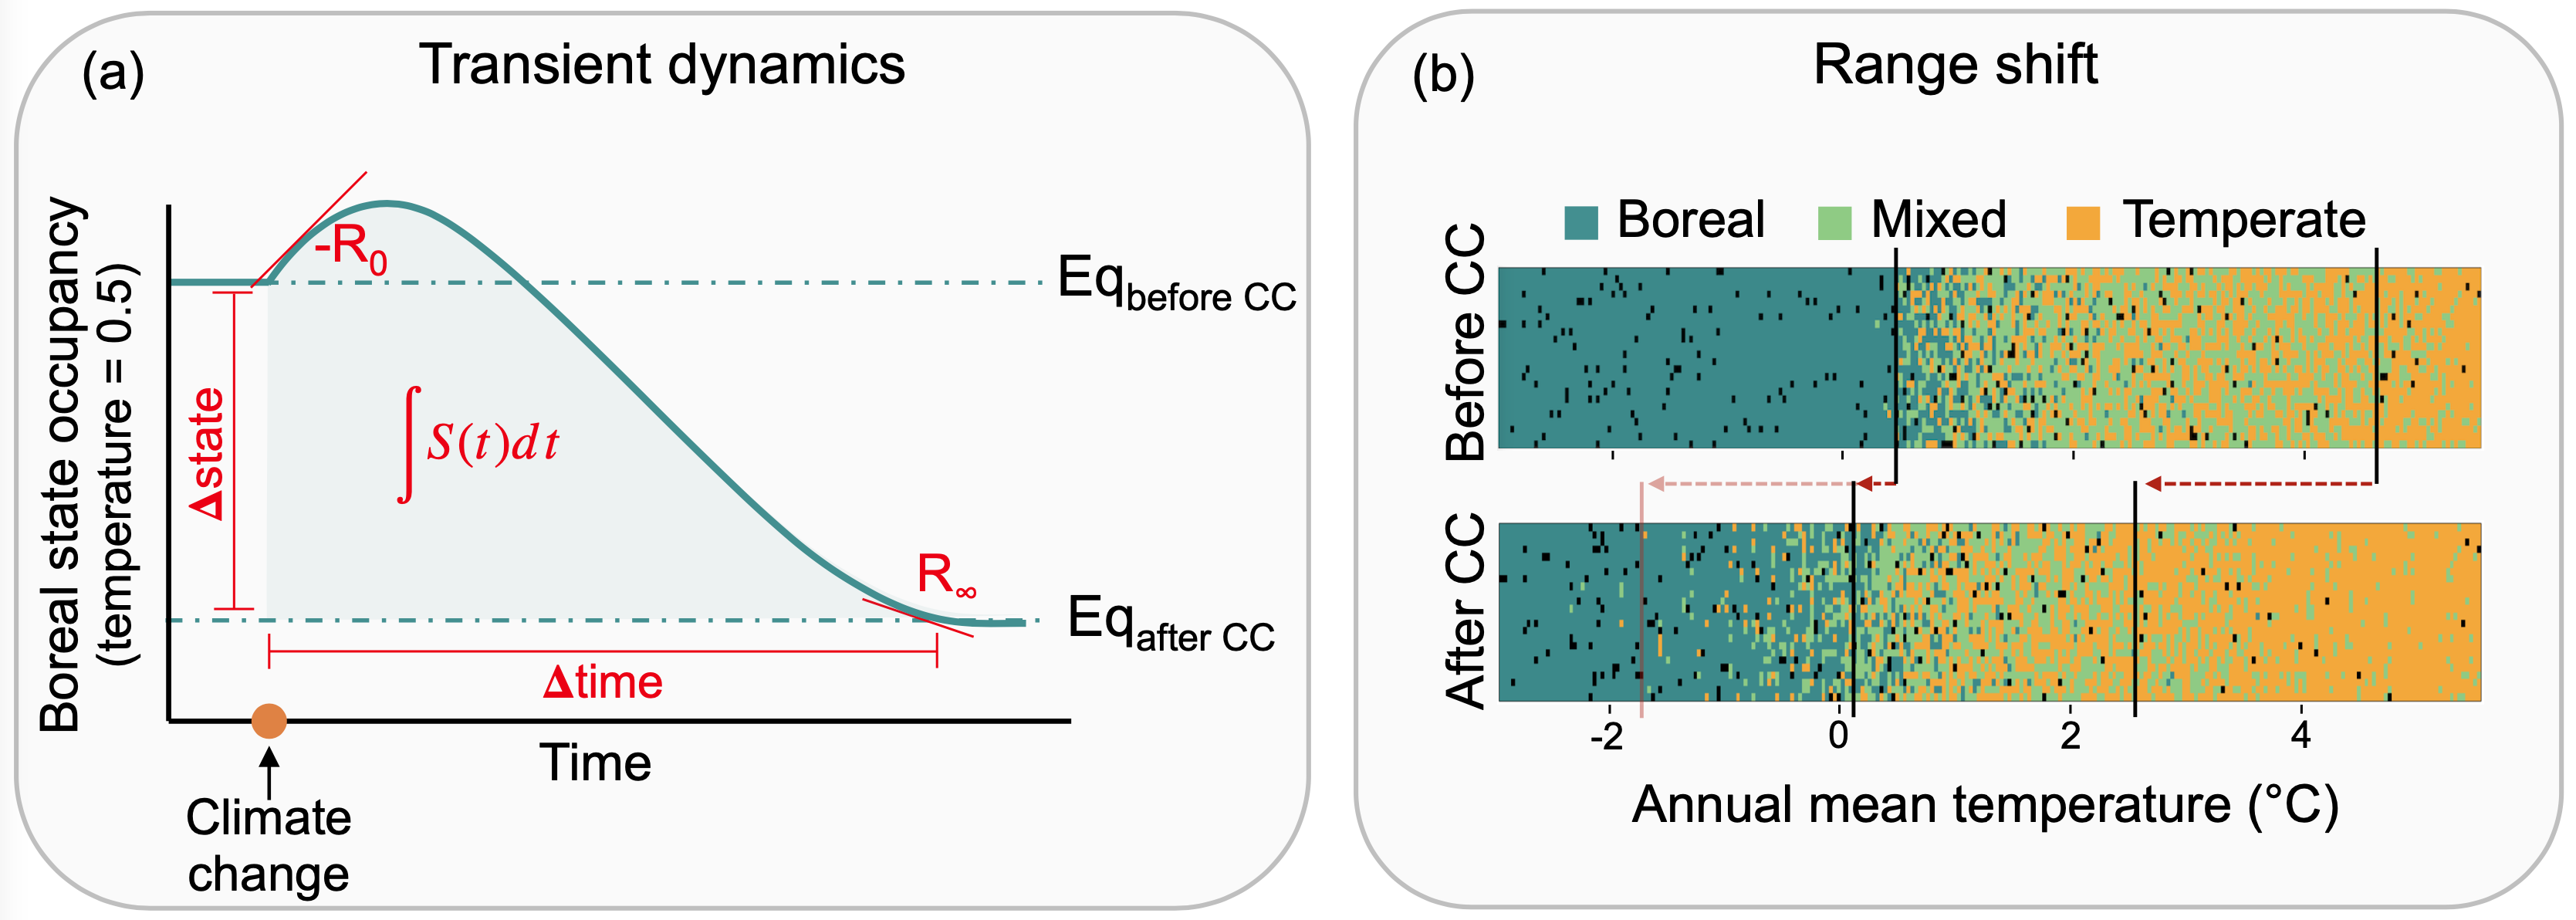
\includegraphics{manuscript/img/concept.png}
\caption[{Conceptual schema of the two approaches used to test the
effect of forest management on the response of forest to temperature
increases.}]{Conceptual schema of the two approaches used to test the
effect of forest management on the response of forest to temperature
increases. (a) Redrawn from \citet{Boulangeat2018}. The spatially
implicit version of the model was used to investigate how forest
management affects the transient dynamics following temperature
increases. Take, for instance, a patch with environmental conditions
that mainly favour boreal species, the increase in temperature due to
climate change will now favour other species over the boreal ones. As a
result, the boreal state occupancy at equilibrium under the new climate
(\(B_1\) at \(t_1\)) will be lower than it was before climate change
(\(B_0\) at \(t_0\)). Five metrics can describe the transient phase
between the old and new equilibrium: initial resilience (\(-R_0\)),
asymptotic resilience (\(R_{\infty}\)), exposure (\(\Delta_{state}\)),
sensitivity (\(\Delta_{time}\)) and cumulative amount of changes
(\(\int S(t)dt\)). (b) The spatially explicit version of the model was
used to study the effect of forest management on the range shift of
forest states following climate change (CC) while accounting for limited
dispersal of trees and stochastic dynamics. The two lattice grids
represent the distribution of pure boreal, mixed, pure temperate, and
regeneration states along a gradient of temperature ranging from boreal
dominant to temperate dominant climate conditions. The cell size of the
grids in this figure was increased for visual clarity. The left and
right vertical black bars indicate the range limit between boreal and
mixed, and between mixed and temperate, respectively. The upper lattice
shows the distribution of forest states in equilibrium with climate
before the increase in temperature (initial state). The bottom lattice
shows, according to \citet{Vissault2020}, that after 150 years following
the increase in temperature, the mixed/temperate range limit followed
climate change (red arrow), but the boreal/mixed range limit did not
(faded red arrow). We use this scenario to study the potential of forest
management to accelerate the range shift of the boreal-temperate ecotone
towards colder temperatures.}
\label{fig:concept}
\end{figure}
}

\hypertarget{modelling-forest-range-limits-and-management-practices}{%
\section{Modelling forest range limits and management
practices}\label{modelling-forest-range-limits-and-management-practices}}

A classical model to study spatial dynamics at the regional spatial
scale comes from Levins' metapopulation theory \citep{Levins1969}. The
theory is particularly suitable to describe the mosaic of forest
successional stages at the landscape scale arising from natural
disturbances and succession. The model describes metapopulation as a set
of patches that are either occupied or empty and connected by dispersal.
At this point, the model is spatially implicit, meaning that dispersal
is global and all patches are connected equally. The dynamics of the
metapopulation is given by individuals arriving and establishing in
empty patches through the process of colonization (\(\alpha\)), and
occupied patches becoming empty through the process of extinction
(\(\varepsilon\)):\\

\begin{equation}
\frac{dp}{dt} = \alpha p (1 - p) - \varepsilon p
\label{eq:metapop}\end{equation}\\

Where \(p\) is the proportion of occupied patches. We can further extend
this model to incorporate an environmental gradient by turning the
demographic parameters (\(\alpha\) and \(\varepsilon\)) into functions
of climate conditions. As a result, we can derive range limits as the
set of environmental conditions where the extinction rate equals the
colonization rate \citep{Holt2005}. Relaxing the assumption of one
single species dynamics, we can consider multiple species competing for
the same patches by having both colonization and extinction parameters
varying as a function of species interactions \citep{Gravel2020}. In
this multi-species setting, range limits are not only determined by
climate, but also by interactions that can either reduce or expand the
northward limit \citep{Godsoe2017}. The theoretical model composed of
differential equations can be made spatially explicit, meaning every
patch is located on a lattice and that dispersal only occurs between
neighboring patches. The spatially explicit model allows us to account
for the effect of dispersal limitations when predicting the response of
trees to climate warming. Our model previously parameterized for eastern
North American forests is derived from this theory \citep{Vissault2020}.\\

Forest landscapes have been conceptualized as a dynamic mosaic of
different states for a long time \citep{PICKETT1985}. While the formal
application of Levins' metapopulation model over a climatic gradient is
recent \citep{Talluto2017}, it builds on key concepts formalized in
previous forest dynamic models. Among the first ones is the description
of successional dynamics with a transition probability matrix by
\citet{horn1971adaptive}. Our approach described bellow is somehow very
similar, with the particularity that the transition matrix is
non-stationary over a climatic gradient and conditional on state
occupancy. \citet{Levin1974} followed not long after with with a model
of disturbances and patch formation used to derive steady-state
distributions of different patch states. Forest gap models like Jabowa
were developped independently \citep{Botkin1972} and later followed by
landscape models like Landis \citep{Mladenoff1996} and its
climate-dependent variant Landis-II \citep{Scheller2004}. Such models,
and other descendants, differ significantly in implementation, scope and
details, but they all share the common feature that landscapes are
composed of patches subject to disturbances (extinction) and succession
(colonization, exclusion) between different states. Our motivation with
the Levins' approach was twofold : i) maintain mathematical tractability
to facilitate its analysis and ii) facilitate model calibration on
forest inventory data. Below we summarize the model conception and
calibration to ease the reading and refer to \citet{Vissault2020} for a
detailed description and sensitivity analysis. We will then develop the
integration of the four management practices in the following section.\\

The State and Transition Model (STM) considers three discrete forest (or
occupied) states along a gradient of temperature: (B)oreal, (T)emperate,
and (M)ixedwood forest states; and the (R)egeneration (or empty) state
\citep{Vissault2020}. The colonization (\(\alpha\)) and extinction
(\(\varepsilon\)) processes drive the transitions between empty (R) and
occupied (by either B, M, or T) patches. The model describes species
interaction through the mechanisms of invasion and competitive
exclusion. Invasion (\(\beta\)) happens when an occupied state type of
pure boreal (B) or pure temperate (T) is colonized by tree species from
the opposite type, and becomes then a mixed state (M). Competitive
exclusion (\(\theta\)) drives the transitions from a mixed forest state
(M) to either state boreal (B) or temperate (T), depending on the
competitive ability of each of forest types. The rate at which occurs
each of these processes (\(\alpha\), \(\varepsilon\), \(\beta\), and
\(\theta\)) is specific to the forest type and the local climatic
conditions, and the resulting process is dependent on the amount of the
corresponding state in the landscape (Figure \ref{fig:model} a).\\

The parameters describing transitions among states were calibrated using
over 40,000 plots from the eastern North American forest
\citep{Vissault2020}. In this study, the database incorporates data from
the FIA in the United States \citep{OConnell2007}, the Canadian
provinces of Québec, Ontario, and New Brunswick
\citep{Naturelles2016, OMNR2014, Porter2001}, as well as a private
forest company in Québec (Domtar). For each plot (measured between 1960
and 2010) and each census, the forest states (B, M, and T) were
classified following their species composition. A stand was classified
as T whenever all boreal species were absent while at least one of the
following eight temperate species was present: \emph{Prunus serotina},
\emph{Acer rubrum}, \emph{Acer saccharum}, \emph{Fraxinus americana},
\emph{Fraxinus nigra}, \emph{Fagus grandifolia}, \emph{Ostrya
virginiana}, and \emph{Tilia americana}. Alternatively, a stand was
classified as B whenever all temperate species were absent while at
least one of the following seven boreal species was present: \emph{Picea
mariana}, \emph{Picea glauca}, \emph{Picea rubens}, \emph{Larix
laricina}, \emph{Pinus banksiana}, \emph{Abies balsamea}, \emph{Thuja
occidentalis}. The stand was classified as mixedwood (M) when both
boreal and temperate species were present. Therefore, T and B stands are
inheritly pure compositions. The stand was classified as regeneration
(R) when the total basal area was inferior to 5 m\(^2\) ha\(^{-1}\),
irrespective of its species composition. After classifying each plot
year into one of the four forest states, transitions were modelled as a
function of local climate conditions, namely mean annual temperature
(MAT) and total annual precipitation (TAP). Parameters of the non-linear
multi-nomial models were evaluated by maximum likelihood and a simulated
annealing optimization procedure. Note that this model avoids the
presumption that the point data is at equilibrium since it predicts the
transition between states rather than the distribution. Only permanent
sampling plots with a time interval within the 5-15 year range were used
in the parameterization (median time interval among plots
\textasciitilde5 years). Furthermore, all disturbances such as fire,
drought, and outbreaks were included in the fitting of the STM; only
managed plots were excluded of the analysis to assure the four
transition processes were naturally induced. Part of the data not used
in the calibration was used to validate the predictions of the model.
The parameters of the model were validated by solving the model to
equilibrium using current climate conditions and comparing the model
predictions to the current forest distribution from the validation data.
The accuracy of the STM in predicting each of the four states given MAT
and TAP ranged from 70\% to 98\% \citep{Vissault2020}.\\

This simple State Transition Model allows one to predict the
distribution of forest community composition at the continental scale.
In the present study, we use the STM equations with their estimated
parameters to integrate the effects of four management practices. We are
aware of the theory that predicts species range limits as a process
derived from their local demographic vital rates
\citep{Araujo2014a, Normand2014}. Given that different species within
the same community have different demographic rates, their response to
climate change will likely generate different range shifts. However,
empirical studies have had little success in establishing the link
between the vital rate of tree species and their distribution
\citep{LeSquin2021, Kunstler2021}. In addition, we can expect that
species within the same forest state will respond similarly to each
other compared to species in other states, regardless of the demographic
variance among the species of the same group. Since we are interested in
exploring how forest management affects forest range limits, we chose to
work beyond the species level to model general management practices at
the scale of forest community composition. Therefore, we stress our
study as a theoretical investigation to guide future models and
experimentation towards adaptive management practices. In the next
section, we detail the ecological assumptions and mathematical
formulation for each management practice implemented in the model.
Finally, with the extended model equations and estimated parameters, we
develop our two simulation approaches to test the effect of forest
management on transient dynamics and forest range shifts.\\

\hypertarget{fig:model}{%
\begin{figure}
\centering
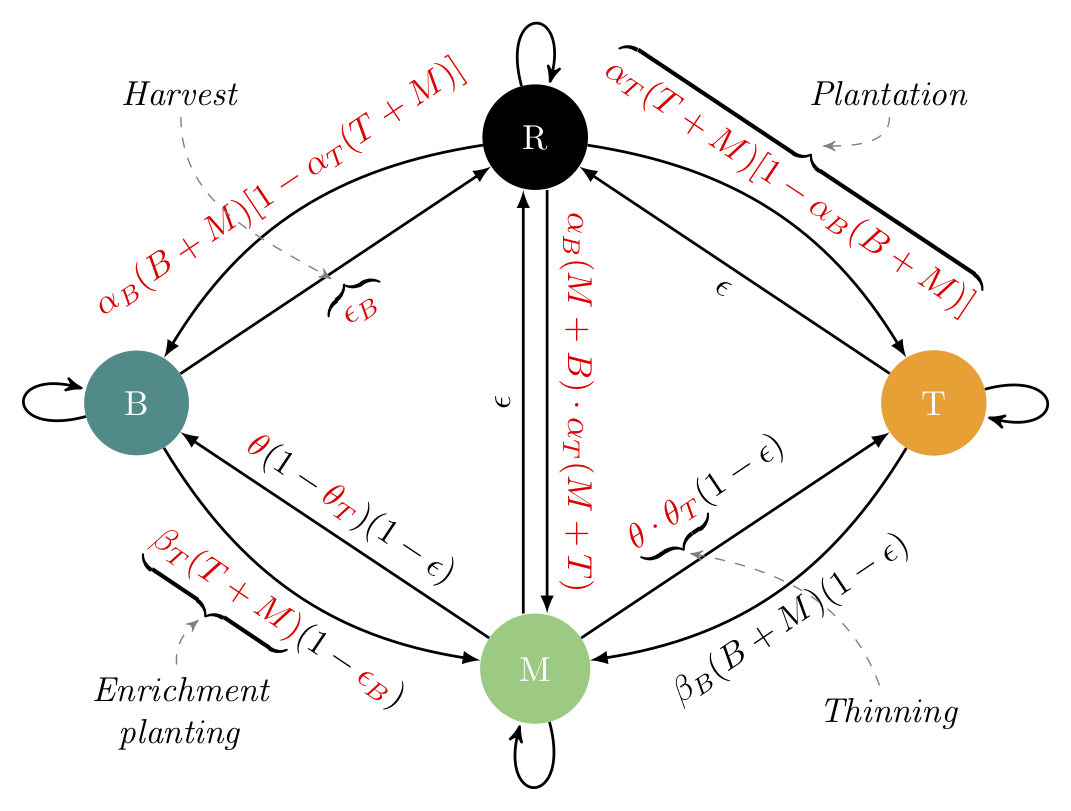
\includegraphics[width=1\textwidth,height=\textheight]{manuscript/img/model_equation_fm.png}
\caption[{Schema of the State and Transition Model adapted from
\citet{Vissault2020}}]{Schema of the State and Transition Model adapted
from \citet{Vissault2020}. Directional arrows describe the colonization
(\(\alpha\)), extinction (\(\varepsilon\)), invasion (\(\beta\)), and
competitive exclusion (\(\theta\)) processes driving the transition
between the four forest states: (R)egeneration, (B)oreal, (T)emperate,
and (M)ixedwood. The panel (b) summarises the effect of increasing the
intensity of forest management in each of the four ecological processes.
For instance, increasing plantation intensity will increase the rate of
transition from R to T and consequently descrease the rate of change
from R to B and from R to M. The values of each of the 9 specific
(process x state) parameters are shown in Figure \ref{fig:sim-result-sup7_ch1}.}
\label{fig:model}
\end{figure}
}

\hypertarget{adapted-forest-management-reducing-the-gap-between-potential-and-actual-forest-distribution}{%
\subsection{Adapted forest management: reducing the gap between
potential and actual forest
distribution}\label{adapted-forest-management-reducing-the-gap-between-potential-and-actual-forest-distribution}}

Given the predictions that the distribution of the boreal-temperate
ecotone may lag behind climate change \citep{Talluto2017, Vissault2020},
here we define and simulate four management practices to test how they
may reduce the gap between potential and realized forest distribution
with climate warming. The four management practices implemented in the
model are plantation and enrichment planting to potentially reduce
colonization credit, and harvest and thinning to potentially reduce
extinction debt. The objective of these management practices is to favor
the migration of both the leading edge of temperate forest and the
trailing edge of boreal forest towards colder temperatures when the
climate is suitable.\\

\hypertarget{forest-management-to-reduce-colonization-credit}{%
\subsubsection{Forest management to reduce colonization
credit}\label{forest-management-to-reduce-colonization-credit}}

Colonization of temperate species beyond the leading edge of their
distribution may depend on many factors such as climate conditions,
competitive ability, and seed sources through dispersion. The first
factor limiting the colonization of a population beyond its range is the
climate. Once the climate limitation is relaxed with climate warming,
species interactions such as competition for light may limit the
development of regenerating individuals \citep[e.g.~][]{Bianchi2018}.
Finally, seed production is a density-dependent process that, associated
with the slow migration rate of trees, contributes to the lack of
colonization beyond the population range limits. In the context of
managing ecological processes, some of these factors can be modified
with forest management. Here we model two management practices that may
operate at different spatial scales to simulate density-independent
colonization: plantation (i.e.~assisted migration) at the large spatial
scale, and enrichment planting at the local spatial scale. Plantation
occurs in regeneration states, while enrichment planting occurs in
mature stands of the alternative composition (e.g.~introducing temperate
hardwoods in a boreal stand). Following temperature increases,
plantation and enrichment planting of temperate species should overcome
dispersal limitation and the lack of seed sources and may increase the
range shift towards colder temperatures by colonizing stands beyond the
current distribution.\\

\hypertarget{plantation-of-temperate-stands}{%
\paragraph{Plantation of temperate
stands}\label{plantation-of-temperate-stands}}

In our model, the establishment of boreal, mixedwood or temperate forest
in regenerating stands depends on the colonization capacity of boreal
and temperate tree species (\(\alpha_B\) and \(\alpha_T\)) as well as
their abundance in the neighboring stands. The plantation practice is
modelled as an increase in the probability of regeneration stands to
become temperate forest stands \(P(T|R)\). A proportion \(p\) of
available stands in state R is thus converted into state T at each time
step. Only the remaining stands in state R (\(1-p\)) are allowed to
follow the natural colonization process. Plantation thus involves an
additional parameter \(p\) that modifies the following probabilities:\\

\begin{equation}
\begin{split}
&P(T|R) = [\alpha_T (T+M) \times (1-\alpha_B (B+M))] \times (1 - p) +  p \\[2pt]
&P(B|R) = [\alpha_B (B+M) \times (1-\alpha_T (T+M))] \times (1 - p) \\[2pt]
&P(M|R) = [\alpha_T (T+M) \times \alpha_B (B+M)] \times (1 - p)
\end{split}
\label{eq:plantation}\end{equation}\\

where \(p\) is the proportion of R stands that are planted per time
step. Note that when \(p=0\), the natural dynamics occurs and when
\(p=1\), \(P(T|R)=1\), \(P(B|R)=P(M|R)=0\).\\

\hypertarget{enrichment-planting-of-temperate-trees-on-boreal-stands}{%
\paragraph{Enrichment planting of temperate trees on boreal
stands}\label{enrichment-planting-of-temperate-trees-on-boreal-stands}}

Invasion of temperate species into boreal stands is a function of the
capacity of temperate forest trees to colonize boreal forest
\(\beta_T\), and the abundance of mixed and temperate in neighboring
stands. Invasion only applies to mature stands. Enrichment planting of
temperate species in boreal stands is modelled as an increase in the
probability of stands in state boreal to become mixedwood \(P(M|B)\).
Among stands in state B available to invasion, a proportion \(e\) is
directly converted to M. The colonization probability of temperate
species establishing in boreal stands after enrichment planting adds a
parameter \(e\) to the model:\\

\begin{equation}
P(M|B) = [(1- (\varepsilon \times (1 - h) + h)) \times \beta_T(T + M)] \times (1-e) + e
\label{eq:enrichplanting}\end{equation}\\

Where \(e\) is the proportion of mature stands in state B that are
enriched at each time step. Natural dynamics occurs when \(e=0\), while
direct conversion by forest management occurs when
\(P(M|B)= 1- (\varepsilon \times (1 - h) + h)\). Note that \(h\) is the
proportion of stands in state B that are harvested as explained in the
next section.\\

\hypertarget{forest-management-to-reduce-extinction-debt}{%
\subsubsection{Forest management to reduce extinction
debt}\label{forest-management-to-reduce-extinction-debt}}

Different ecological mechanisms can explain extinction debt caused by
the delayed response of forest trees to temperature increases. Slow
demographic rates along with dispersal limitations can delay the
response of species to environmental changes \citep{Dullinger2012}.
These life-history traits, associated with source-sink dynamics
\citep{Schurr2012}, can increase considerably the extinction debt of
tree populations following temperature increases. To reduce this delayed
response, unadapted species would have to disappear and therefore make
room for the new species that is better adapted to the novel
environmental conditions. Disturbance and competitive exclusion are two
ecological processes suitable to influence the rate of extinction and,
if well directed, reduce extinction debt. Here we chose harvest and
thinning, which is a partial harvest within a stand, as complementary
management practices that may accelerate disturbance and competitive
exclusion. Harvest of stands in state B has the same effect than large
spatial scale disturbances, such as fire, and transform a proportion of
B stands in a R state. Similarly, removal of boreal species by selective
thinning in stands of state M can increase the rate at which temperate
species can competitively exclude boreal species. Both harvest and
thinning are intended to open space and reduce the proportion of boreal
species, and therefore increase the likelihood of temperate states to
shift towards colder temperatures.\\

\hypertarget{harvest-of-boreal-stands}{%
\paragraph{Harvest of boreal stands}\label{harvest-of-boreal-stands}}

In the natural extinction model, stands in state B turn into a
regeneration state only after natural disturbances, occurring at a
probability \(\varepsilon\). Harvest is modelled as an increase in the
probability of boreal states to become regeneration states \(P(R|B)\). A
proportion \(h\) of mature stands in state B is converted into state R,
featuring the cut of all trees. This proportion of B stands is thus
excluded from following natural dynamics. Harvest thus involves an
additional parameter \(h\) that modifies the following probabilities:\\

\begin{equation}
\begin{split}
&P(R|B) = [\varepsilon \times (1 - h)] + h \\[2pt]
&P(M|B) = (1- (\varepsilon \times (1 - h) + h)) \times \beta_T(T + M)
\end{split}
\label{eq:harvestEq}\end{equation}\\

Where \(h\) is the proportion of stands in state B that are harvested at
each time step. If \(h=1\), no B stands will be maintained, and when
\(h=0\), only natural disturbance occurs.\\

\hypertarget{thinning-of-boreal-trees-in-mixedwood-stands}{%
\paragraph{Thinning of boreal trees in mixedwood
stands}\label{thinning-of-boreal-trees-in-mixedwood-stands}}

In the natural model, the transition from a mixed state M to either a
pure state (B or T) is driven by the instability of the state M
(\(\theta\)), and the competitive ratio between temperate and boreal
species (\(\theta_T\)). It means that the higher the instability
(\(\theta\)), the higher the probability of competitive exclusion, and
the winner is given the competitive ratio between temperate and boreal
species (\(\theta_T\)). Thinning of boreal species in M stands is
modelled as an increase of the probability of M stands to become state T
in two different ways (\(s_1\) and \(s_2\)). First, thinning of boreal
species can be translated into an increase in the instability of M
stands:\\

\begin{equation}
  \theta_{m} = [\theta \times (1 - s_1)] + s_1
\label{eq:thinningEq}\end{equation}\\

Second, selective thinning of boreal species can increase the
competitive ability of temperate species:\\

\begin{equation}
\theta_{T, m} = [\theta_{T} \times (1 - s_2)] + s_2
\label{eq:thinningEq2}\end{equation}\\

It is unclear if we need to distinguish between the two processes. The
rationale is that the proportion \(s_1\) of M stands that are managed
this way is directly converted into state T. It means that \(s_2\)
should at least be equal to \(s_1\). If thinning further boost the
competitivity (fitness) of temperate species, then \(s_2\) can be
greater than \(s_1\). For a parsimonious approach, it seems reasonable
to set \(s_1=s_2\). These modifications directly affect \(P(T|M)\) and
\(P(B|M)\):\\

\begin{equation}
\begin{split}
&\theta_{m} = [\theta \times (1 - s)] + s \\[2pt]
&\theta_{T, m} = [\theta_{T} \times (1 - s)] + s \\[2pt]
&P(T|M) = \theta_m \times \theta_{T,m} \times (1 - \varepsilon) \\[2pt]
&P(B|M) = \theta_m (1 - \theta_{T,m}) \times (1 - \varepsilon)
\end{split}
\label{eq:thinningEq3}\end{equation}\\

Where \(s\) is the proportion of undisturbed stands in state M where
thinning is applied per time step. When \(s=1\), \(P(T|M) = 1\) and
\(P(B|M) = 0\).\\

\hypertarget{simulation-analysis}{%
\subsection{Simulation analysis}\label{simulation-analysis}}

\hypertarget{analysis-of-the-transient-dynamics-under-climate-warming}{%
\subsubsection{Analysis of the transient dynamics under climate
warming}\label{analysis-of-the-transient-dynamics-under-climate-warming}}

We used the spatially implicit version of the STM at equilibrium with
current climate conditions to test the effect of forest management on
the transient dynamics following temperature increases. To do so, we
simulated an increase in temperature and focused on the dynamics of the
transient period of the four forest states until they reach the new
steady state. Steady state was considered as being reached when the
difference between two successive states prevalence was inferior to
\(10^{-7}\) for 10 consecutive steps. Each step in the model is equal to
5 years according to the initial parameterization of the model
\citep{Vissault2020}. We characterized the transient dynamics over a
gradient of mean annual temperature ranging from -2.61 to 5.07
\(^{\circ}\)C. Note that this approach quantifies the model's local
stability for a specific location defined by climatic conditions. As a
result, no spatially explicit dynamics like dispersal are considered,
and the transient metrics are calculated separately for each location
along the MAT gradient. This gradient corresponds to the current
temperature range along with the temperate-to-boreal forest ecotone, and
it is the reason we describe this gradient as ``initial mean annual
temperature''. This gradient can be visualized by drawing a straight
line from Montreal (\textasciitilde45.5 \(^{\circ}\) N) to Chibougamau
(\textasciitilde49.9 \(^{\circ}\) N), in Canada. While we simulated
temperature changes, TAP was kept constant to the mean value extracted
from the database (998.7 mm) because TAP has a relatively small effect
on model outputs compared to MAT \citep{Vissault2020}. Temperature
increased by 0.09 \(^{\circ}\)C at each time step for the first 20 steps
(100 years) for a total increase of 1.8 \(^{\circ}\)C following the
Representative Concentration Pathway (RCP) scenario of 4.5, and then
remained constant until the model reached the steady state. As we used a
linear increase of temperature to represent the boreal-temperate ecotone
(ranging from -2.61 to 5.07 \(^{\circ}\)C) instead of a real landscape,
the RCP scenarios are based on the mean global projections
\citep{IPCC2013}. We further tested the RCP8.5 scenario and observed
that the increase in the disturbance intensity with warmer temperatures
only shifted the reponse to higher values, but did not change the
overall interpretation compared to RC4.5 (results not shown).\\

We characterized the transient phase after temperature increases using
five different metrics from \citet{Boulangeat2018}. The first two
metrics are the asymptotic and initial resilience as measures of local
stability derived from the Jacobian Matrix \(J\) at the new equilibrium
\citep{Arnoldi2016}. \(J\) was numerically calculated using the R
package rootSolve \citep{Soetaert2009, Soetaert2009a}. The asymptotic
resilience (\(R_{\infty}\)) is the leading eigenvalue of \(J\), and
quantifies the asymptotic rate of return to equilibrium after small
perturbation. The more negative \(R_{\infty}\), the greater is the
asymptotic rate of change back to the equilibrium, and therefore the
greater the resilience of the system. Although the stability metrics are
computed at the new equilibrium, we can derive the initial reactivity of
the system to disturbance using algebra transformation of the matrix
\(J\) \citep{Neubert1997}. Initial resilience (\(-R_0\)), defined by
\citet{Arnoldi2016} as the inverse of initial reactivity, is the leading
eigenvalue of the following matrix:\\

\begin{equation}
M = \frac{-J + J^T}{2}
\label{eq:jacob}\end{equation}\\

Positive values of \(-R_0\) indicate a smooth transition to the new
equilibrium whereas negative values indicate reactivity, that is, an
initial amplification in the opposite direction to the final
equilibrium. The third metric is the exposure of the ecosystem states
(\(\Delta_{state}\)), defined by the euclidean distance between initial
and final state prevalence among the four states \citep{Dawson2011}. It
reports the amount of change the system will experience. The fourth
metric is the return time (\(\Delta_{time}\)) or ecosystem sensitivity,
which is estimated by the number of time steps of the transitory phase.
A combination of the previous metrics, it describes how long it takes to
reach the new equilibrium. The last metric is the cumulative amount of
changes in the transitory phase, or ecosystem vulnerability
\citep{Boulangeat2018}. It is defined as the sum of all changes in the
states after climate warming and is obtained by the integral of the
states change over time (\(\int S(t)dt\)). It combines all of the prior
metrics to describe how much the system is ``out-of-equilibrium'' or
vulnerable. These five metrics together can summarize the
multidimensionality of the response of a system to external
disturbances.\\

We used five distinct simulation scenarios: natural dynamics without
forest management, 0.25\% of plantation, 0.25\% of enrichment planting,
1\% of harvest, and 0.25\% of thinning, at an annual rate. The above
values were chosen to maintain a certain degree of realism. In the
Canadian province of Quebec, about 1\% of the forest territory is
harvested annually. Of this 1\% harvested, only 20 to 25\% is followed
by planting. To our knowledge, enrichment planting and thinning of a
specific species are more complex to operate and rarely used in Quebec
and should not overpass the other practices, hence we chose to analyze
the same amount as the plantation. To further quantify the effect of
increasing the intensity of forest management from 0 to 100\% for each
practice. For instance, increasing plantation to 100\% (\(p = 1\)) means
that all regeneration stands will become T. For that, we chose two
locations from the gradient of temperature in which forest management
had the most effect on the metrics of transient dynamics: -1 and 0
\(^{\circ}\)C MAT which represents the leading and trailing edge of the
ecotone.\\

\hypertarget{analysis-of-the-range-shift-under-climate-warming}{%
\subsubsection{Analysis of the range shift under climate
warming}\label{analysis-of-the-range-shift-under-climate-warming}}

Using the model equations with forest management, we created a spatially
explicit version of the model with an artificial landscape (lattice) to
account for explicit dispersal limitations and stochastic dynamics, to
test the capacity of forest management to accelerate the range shift of
the boreal-temperate ecotone towards colder temperatures. The landscape
is composed as a regular grid of 1698 by 170 cells where each cell
(approx. 300 x 300 meters) at each time step is occupied by one of the
four forest states (R, B, T or M). Given the average dispersal rate for
some temperate trees is in the range of 5-15 \(m \cdot yr^{-1}\)
\citep{Ribbens1994}, with maximum dispersal rates estimated in the
post-glacial period reaching 260 \(m \cdot yr^{-1}\)
\citep{Feurdean2013}, our 300 m grid has sufficient distance to account
for the rare long-distance dispersal events. Sensitivity analysis showed
that the range shift following climate warming increased with larger
grid cells (from 1 hectare to 2500 hectares), but the effect was
stronger in cells larger than 100 hectares (Figure \ref{fig:sim-result-supp1_ch1}). While the choice
of the cell size affects the absolute value of range shift, it does not
affect the relative effect of the different forest management
strategies. Moreover, although the smaller the cell the better we model
dispersion, smaller cells are computationally expensive. Therefore, the
size of 300 x 300 m (9 ha) was the best compromise between these two
factors. The gradient of the landscape grid was defined using the same
MAT range as in the spatially implicit model (-2.61 to 5.07
\(^{\circ}\)C) to represent the whole ecotone from boreal to temperate
dominant forest types, with a constant TAP of 998.7 mm. The prevalence
of each state at time \(t + 1\) was calculated considering the stand
composition of the eight neighboring cells and the temperature and
precipitation condition of the cell at time \(t\). The state of the
current cell at time \(t + 1\) was then randomly drawn from the
transition probabilities. The effect of climate warming on the landscape
dynamics was simulated by increasing temperature of 0.09 \(^{\circ}\)C
for each cell at each time step for the first 20 steps (100 years;
RCP4.5). We further performed simulations using the RCP8.5 scenario, and
the results are shown in Figure \ref{fig:sim-result-supp6_ch1}. The spatially explicit version of
the model was bind into an R package stored on GitHub
\citep{STManaged2020}. We used the released version v2.0 of the package
to run the simulations for this article.\\

We ran three simulations to compare the relative importance of
temperature increases, forest management, and their interaction with the
equilibrium distribution in future climate conditions. The intensity of
the four management practices was the same as used in the first
approach, and they were equally applied across the landscape. The model
simulated 150 years of forest dynamics under three different scenarios:
(i) only climate change, (ii) only one forest management practice, and
(iii) climate change and one forest management practice at a time. These
``virtual experimental treatments'' allow to independently characterize
their independent effects and also their interaction. These three
simulation scenarios were then compared with current (\(T_0\)) and
future (\(T_1\)) forest distribution at equilibrium with climate as
reference points. For each simulation and reference points, we
quantified the boreal and the mixed/temperate occupancy over the
gradient of initial mean annual temperature (-2.61 to 5.07
\(^{\circ}\)C). This allowed us to visualize the response of state
occupancy to each simulation. In addition, we computed the average range
shift of state occupancy in mean annual temperature for each simulation,
taking the initial distribution at equilibrium with climate (\(T_0\)) as
the starting point. Range shift represents the shift of state occupancy
relative to the initial mean annual temperature. This approach allowed
us to quantify the displacement of the boreal-temperate ecotone in the
grid without the need of arbritary thresholds to define the range limits
of a forest type. Range shift was calculated as the difference in
initial mean annual temperature between the first and final step of a
simulation run for all values of state occupancy ranging from 0 and 1.
We removed extreme values of state occupancy (\(state_{occ} < 0.07\);
\(state_{occ} > 0.93\)) to avoid miscalculation of range shift as our
approach was imprecise in these extreme locations. This filter had
little effect on the median and quantiles of range shift (Figure \ref{fig:sim-result-supp2_ch1}).
Negative values of range shift indicate a displacement of the
distribution of a forest type towards colder temperatures, whereas
positive values indicate a displacement towards warmer temperatures.\\

Finally, as the chosen time scale (150 years) and management intensity
may not be large enough to detect the response of forests to temperature
increases and forest management, we ran the same configuration of
simulations while increasing both the time scale and the management
intensity. The running time of each simulation was increased to 250, 500
and 1000 years, and management intensity for all practices increased to
2, 5, 10 and 20\%. We replicated the simulations 15 times, while varying
the initial landscape for each simulation. Initial landscapes were
randomly generated, with the prevalence of each cell determined by the
MAT value across the gradient of the lattice grid.\\

\hypertarget{results}{%
\section{Results}\label{results}}

\hypertarget{effect-of-forest-management-on-transient-dynamics-under-climate-warming}{%
\subsection{Effect of forest management on transient dynamics under
climate
warming}\label{effect-of-forest-management-on-transient-dynamics-under-climate-warming}}

We characterized the transient dynamics following an increase of 1.8
\(^{\circ}\)C in temperature along the boreal-temperate ecotone.
Overall, all metrics peaked in two specific regions, indicating maximum
resilience at the transition between boreal and mixedwood
(\textasciitilde{} -1 \(^{\circ}\)C), and at the transition between
mixedwood and temperate dominant forest types (\textasciitilde{} 3
\(^{\circ}\)C; Figure \ref{fig:num-res1} a for reference). Plantation
and enrichment planting of temperate species, which simulate the payment
of colonization credit, were the only two practices affecting
significantly the transient dynamics following climate warming. The
effect of these two practices on the transient metrics was observed only
in the transitional region between boreal and mixedwood. Exposure
increased with enrichment planting in the boreal region (Figure
\ref{fig:num-res1} b), meaning that forest management promoted the shift
of forest states to a new equilibrium. The time for the forest to reach
the new equilibrium following climate warming (sensitivity) was reduced
by about 40 and 80\% with plantation and enrichment planting,
respectively (Figure \ref{fig:num-res1} c). The cumulative state changes
(Figure \ref{fig:num-res1} d) integrates the variation in both exposure,
sensitivity, and resilience into a single metric, ecologically
interpreted as ecosystem vulnerability. In the transition between boreal
and mixedwood states, where vulnerability is at its peak, plantation and
enrichment planting reduced vulnerability by 55 and 78\%, respectively.
In both transition regions between dominant forest types, asymptotic
resilience was close to zero, meaning a weak resilience of the system
due to its slow rate of change following a perturbation (Figure
\ref{fig:num-res1} e). In the same locations, initial resilience was at
its peak, meaning that the system is less reactive to a disturbance
(Figure \ref{fig:num-res1} f). This means that the forest ecosystem has
a slow reaction at the beginning and/or at the end of the transient
phase (see Figure \ref{fig:concept} a for a visual interpretation).
Enrichment planting was the only practice to change both resilience
metrics, doubling asymptotic resilience, and reducing initial resilience
by 13\%. Reducing colonization credit through plantation and enrichment
planting of temperate species were effective in changing the transient
dynamics under temperature increases, helping forest to keep pace with
climate change.\\

\hypertarget{fig:num-res1}{%
\begin{figure}
\centering
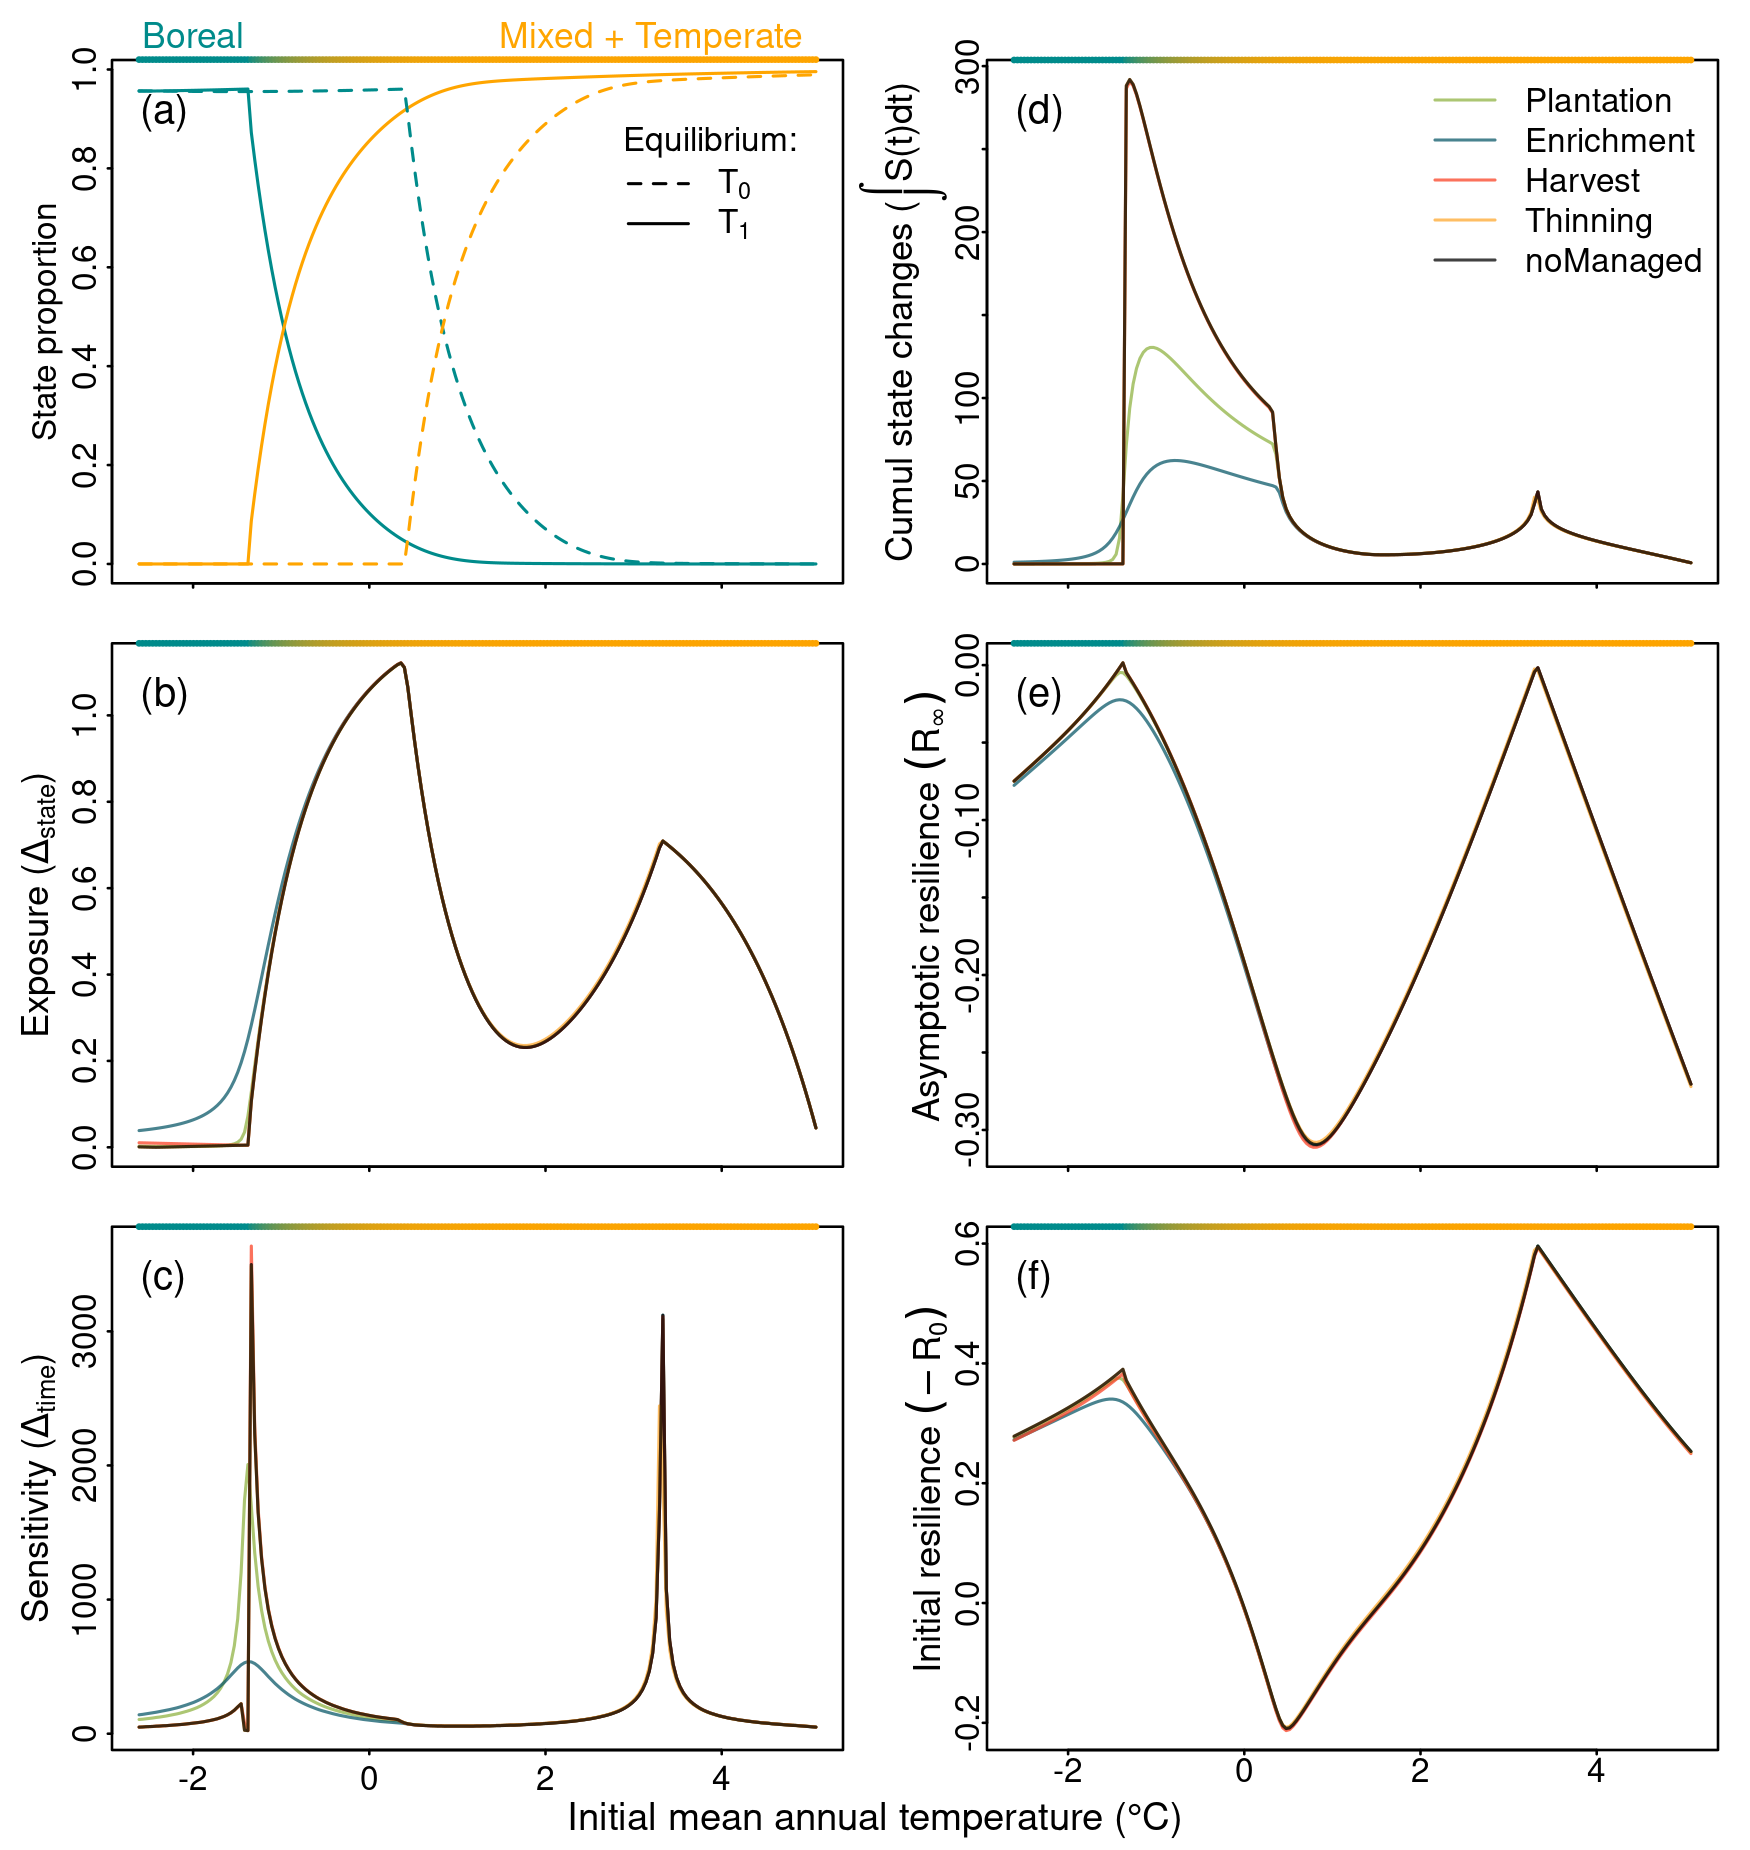
\includegraphics[width=0.9\textwidth,height=\textheight]{manuscript/img/num-result.png}
\caption[{Expected occupancy of boreal and temperate-mixed states at
equilibrium with climate before (\(T_0\)) and after (\(T_1\))
temperature increases (RCP4.5) as a climatic reference}]{Expected
occupancy of boreal and temperate-mixed states at equilibrium with
climate before (\(T_0\)) and after (\(T_1\)) temperature increases
(RCP4.5) as a climatic reference (a). (b-f) Transient dynamics following
climate warming along the gradient of mean annual temperature for five
different scenarios: natural dynamics without forest management, 0.25\%
of plantation, 0.25\% of enrichment planting, 1\% of harvest and 0.25\%
of thinning. Transient dynamics are described by (b) exposure or the
shift of forest states to the new equilibrium; (c) sensitivity or the
time for the state reach equilibrium after climate warming; (d)
vulnerability or the cumulative amount of state changes after
temperature increases; (e) asymptotic resilience or the rate in which
the system recovery to equilibrium; and (f) initial resilience or the
reactivity of the system after temperature increases.}
\label{fig:num-res1}
\end{figure}
}

Given that the effect of forest management on the transient metrics was
stronger in the transitional region between boreal and mixedwood state
dominance (Figure \ref{fig:num-res1}), we selected two contrasting
locations in this region to evaluate the effect of increasing forest
management intensity on the transient metrics (Figure
\ref{fig:num-res2}). Enrichment planting and plantation remained the two
practices with the greatest effect on the transient metrics, increasing
exposure and resilience, and decreasing the return time (sensitivity) in
the boreal region (at -1\(^{\circ}\)C; figure \ref{fig:num-res2} a-c).
Moreover, the effect of these two practices was non-linear, thus a small
increase in management intensity had a large effect on the transient
metrics. For instance, a 20\% increase in enrichment planting will
increase exposure to 90\% to its maximum (Figure \ref{fig:num-res2} a),
and reduce asymptotic resilience (Figure \ref{fig:num-res2} b) and
sensitivity (Figure \ref{fig:num-res2} c) to 70\% of their maximum. The
increase in harvesting intensity of boreal stands also increased the
exposure and sensitivity of the system (Figure \ref{fig:num-res2} c).
Similarly, increasing thinning intensity in mixedwood stands increased
exposure and sensitivity (Figure \ref{fig:num-res2} d, f) but reduced
resilience (Figure \ref{fig:num-res2} e). Increasing management
intensity can accelerate forest response to climate change through
enrichment planting or plantation, but it can also delay this response
through harvesting and thinning. Initial resilience and cumulative state
changes are omitted in the Figure \ref{fig:num-res2}, and can be found
in the supporting information (Figure \ref{fig:sim-result-supp3_ch1}).\\

\hypertarget{fig:num-res2}{%
\begin{figure}
\centering
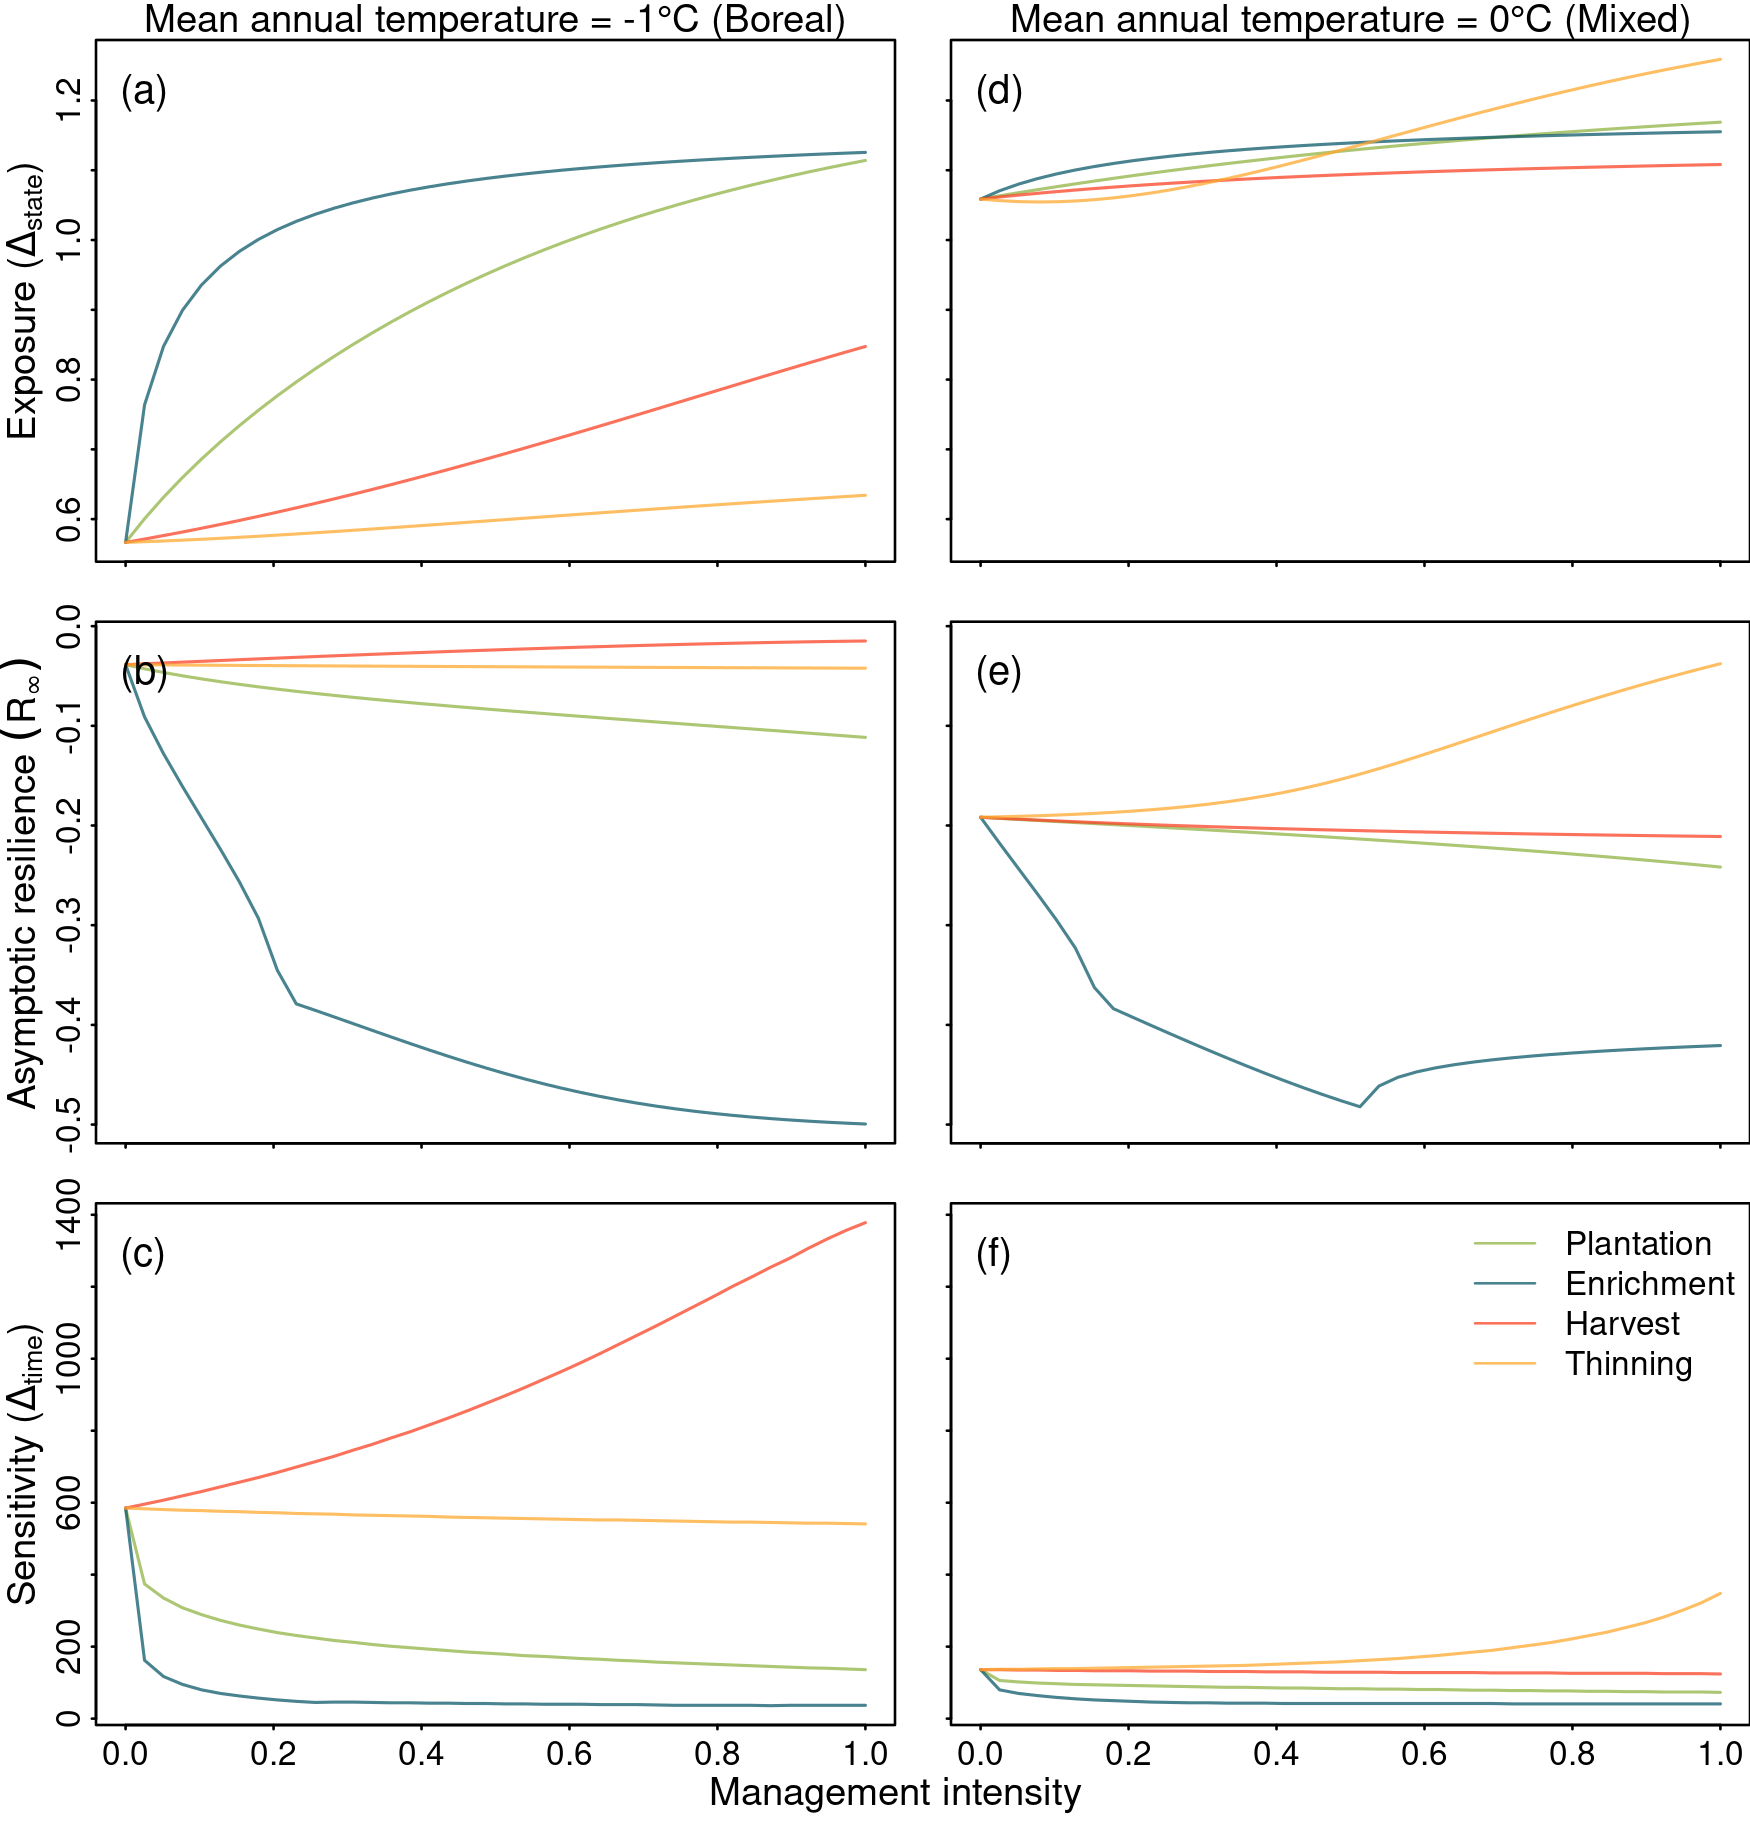
\includegraphics{manuscript/img/num-result_2.png}
\caption[{Effect of increasing management intensity on the transient
metrics characterizing how the model responds to climate warming
(RCP4.5)}]{Effect of increasing management intensity on the transient
metrics characterizes how the model responds to climate warming
(RCP4.5). The effect of increasing management intensity is observed on
two specific climate conditions represented by the initial mean annual
temperature: -1 (dominated by boreal; left panels) and 0 (boreal/mixed
state ecotone; right panels) regions. Transient dynamics are described
by (i) exposure or the shift of forest states to the new equilibrium;
(ii) asymptotic resilience or the rate at which the system recovers to
equilibrium; and (iii) sensitivity or the time for the state to reach
equilibrium after climate warming. Details on each metric are described
in Figure \ref{fig:num-res1}}
\label{fig:num-res2}
\end{figure}
}

\hypertarget{effect-of-forest-management-on-range-limit-shift-under-climate-warming}{%
\subsection{Effect of forest management on range limit shift under
climate
warming}\label{effect-of-forest-management-on-range-limit-shift-under-climate-warming}}

We investigated how forest management affects the range limit shift
between the the boreal trailing edge and the mixed leading edge using
spatially explicit simulations accounting for dispersal limitations and
stochastic dynamics. Given the state distribution dominance at
equilibrium with current climate (light shaded area in Figure
\ref{fig:sim-result}), we expect climate warming to push the forest
distribution towards colder temperatures with a median range shift of
-1.8 \(^{\circ}\)C (which corresponds to the simulated temperature
increase, dark shaded area in Figure \ref{fig:sim-result} and dashed
line in Figure \ref{fig:sim-result2} b). After 150 years with no
management and no climate change, the boreal and temperate+mixed forest
dominance slightly shifted towards warmer temperatures with a median
range shift of 0.10 \(^{\circ}\)C, the same rate when plantation,
harvest, and thinning were applied (Figure \ref{fig:sim-result2} a).
Enrichment planting with no climate change shifted the dominance of the
boreal-temperate ecotone towards colder temperatures with a median range
shift of -0.03 \(^{\circ}\)C. After 150 years with climate warming
following the RCP4.5 scenario, the range of boreal and temperate+mixed
shifted only -0.53 \(^{\circ}\)C, contrary to the expected -1.8
\(^{\circ}\)C (Figure \ref{fig:sim-result2} b). Furthermore, we can
observe under RCP4.5 without forest management that the slope of the
transition between boreal and temperate+mixed forest dominance increased
with climate warming, meaning that the smooth transition observed at the
initial condition (light shaded area) became a more abrupt transition
between these two forest types (Figure \ref{fig:sim-result}). In this
RCP scenario, neither plantation, harvest, nor thinning had a
significant effect on range shift compared to the unmanaged scenario
(Figure \ref{fig:sim-result2} b). Enrichment planting was the single
practice to increase range shift towards colder temperature with a
median of -1.31 \(^{\circ}\)C. Reducing colonization credit, through
enrichment planting, increased the range shift of the boreal-temperate
ecotone when interacting with climate change, creating a smooth
transition between the dominance of these two forest types.\\

\hypertarget{fig:sim-result}{%
\begin{figure}
\centering
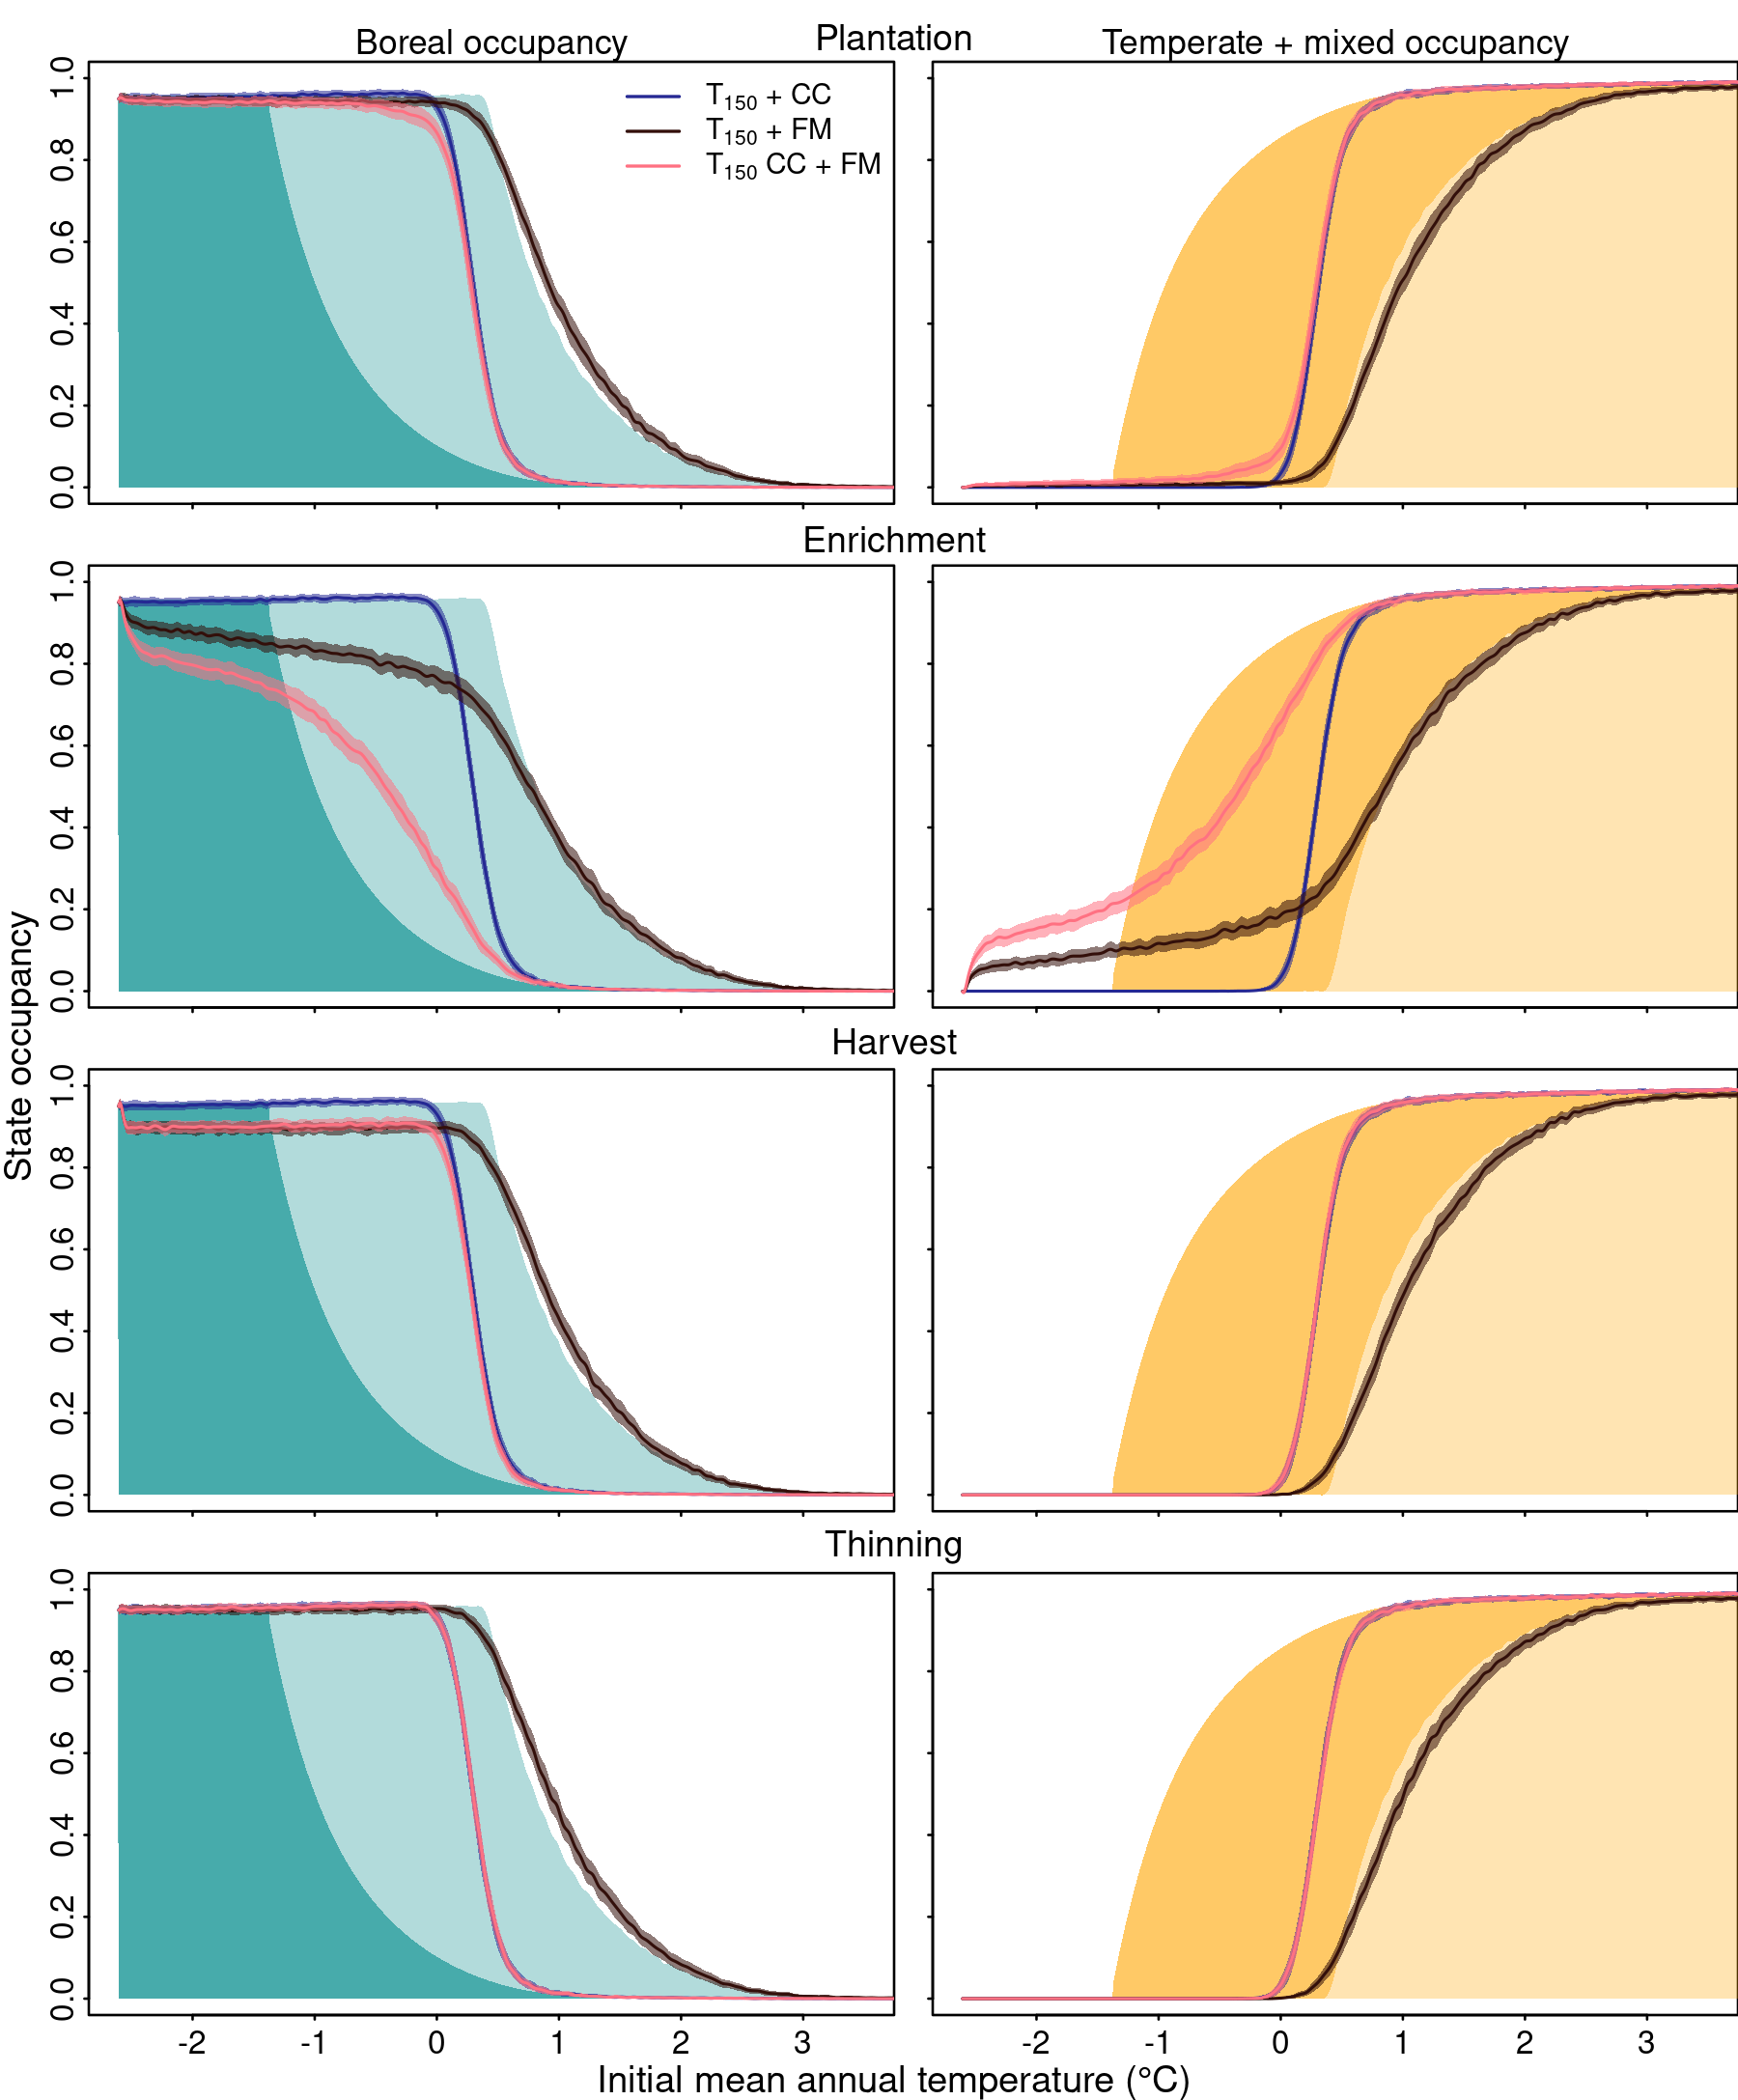
\includegraphics[width=0.79\textwidth,height=\textheight]{manuscript/img/sim-result_RCP4.5.png}
\caption[{Boreal (left panels) and mixedwood/temperate (right panels)
occupancy across the landscape grid covering the boreal-temperate
ecotone.}]{Boreal (left panels) and mixedwood/temperate (right panels)
occupancy across the landscape grid covering the boreal-temperate
ecotone. State occupancy is the proportion of that state for a given
location of initial mean annual temperature in the landscape grid. Note
that because we are more interested in the boreal/mixed range limit, we
chose to simplify the figure by considering the mixed and temperate
states together. Light and dark shaded areas are a reference of the
state occupancy in the landscape at equilibrium before and after
temperature increases, respectively. We ran our model for 150 years
(T150) under three alternative scenarios: only climate change (CC), only
forest management (FM), and climate change with forest management (CC +
FM) to assess their interactions. The results are the mean and 99\%
confidence intervals of 15 replicates. Management intensity was set to
0.25\% for plantation, thinning, and enrichment planting, and 1\% for
harvest. The climate change scenario was RCP 4.5.}
\label{fig:sim-result}
\end{figure}
}

Simulation time and management intensity of figure \ref{fig:sim-result}
and \ref{fig:sim-result2} were kept small for the sake of realism, but
we further tested how increasing these two parameters will affect range
shift of the boreal-temperate ecotone. Overall, increasing the
simulation time increases range shift towards colder temperatures,
approaching the expected equilibrium under the RCP4.5 scenario (Figure
\ref{fig:sim-result3} a-c; Figure \ref{fig:sim-result-supp4_ch1}). After 250 years of simulation,
enrichment planting shifted the distribution of the boreal-temperate
ecotone with a median of -1.71 \(^{\circ}\)C, nearly reaching the
expected equilibrium of -1.8 \(^{\circ}\)C (Figure \ref{fig:sim-result3}
a). The remaining management practices did not have a strong effect on
range shift, with a shared median between plantation, harvest, and
thinning around -0.85 \(^{\circ}\)C, compared with -0.79 \(^{\circ}\)C
when no management was applied. After 500 years of simulation, both
enrichment planting and plantation differed from the other practices,
with a median range shift of -1.85 \(^{\circ}\)C and -1.43
\(^{\circ}\)C, respectively (Figure \ref{fig:sim-result3} b). After a
thousand years, enrichment planting remained stable for 500 years, and
all the other practices almost reached the expected equilibrium, with a
median range shift around -1.59 \(^{\circ}\)C (Figure
\ref{fig:sim-result3} b).\\

\hypertarget{fig:sim-result2}{%
\begin{figure}
\centering
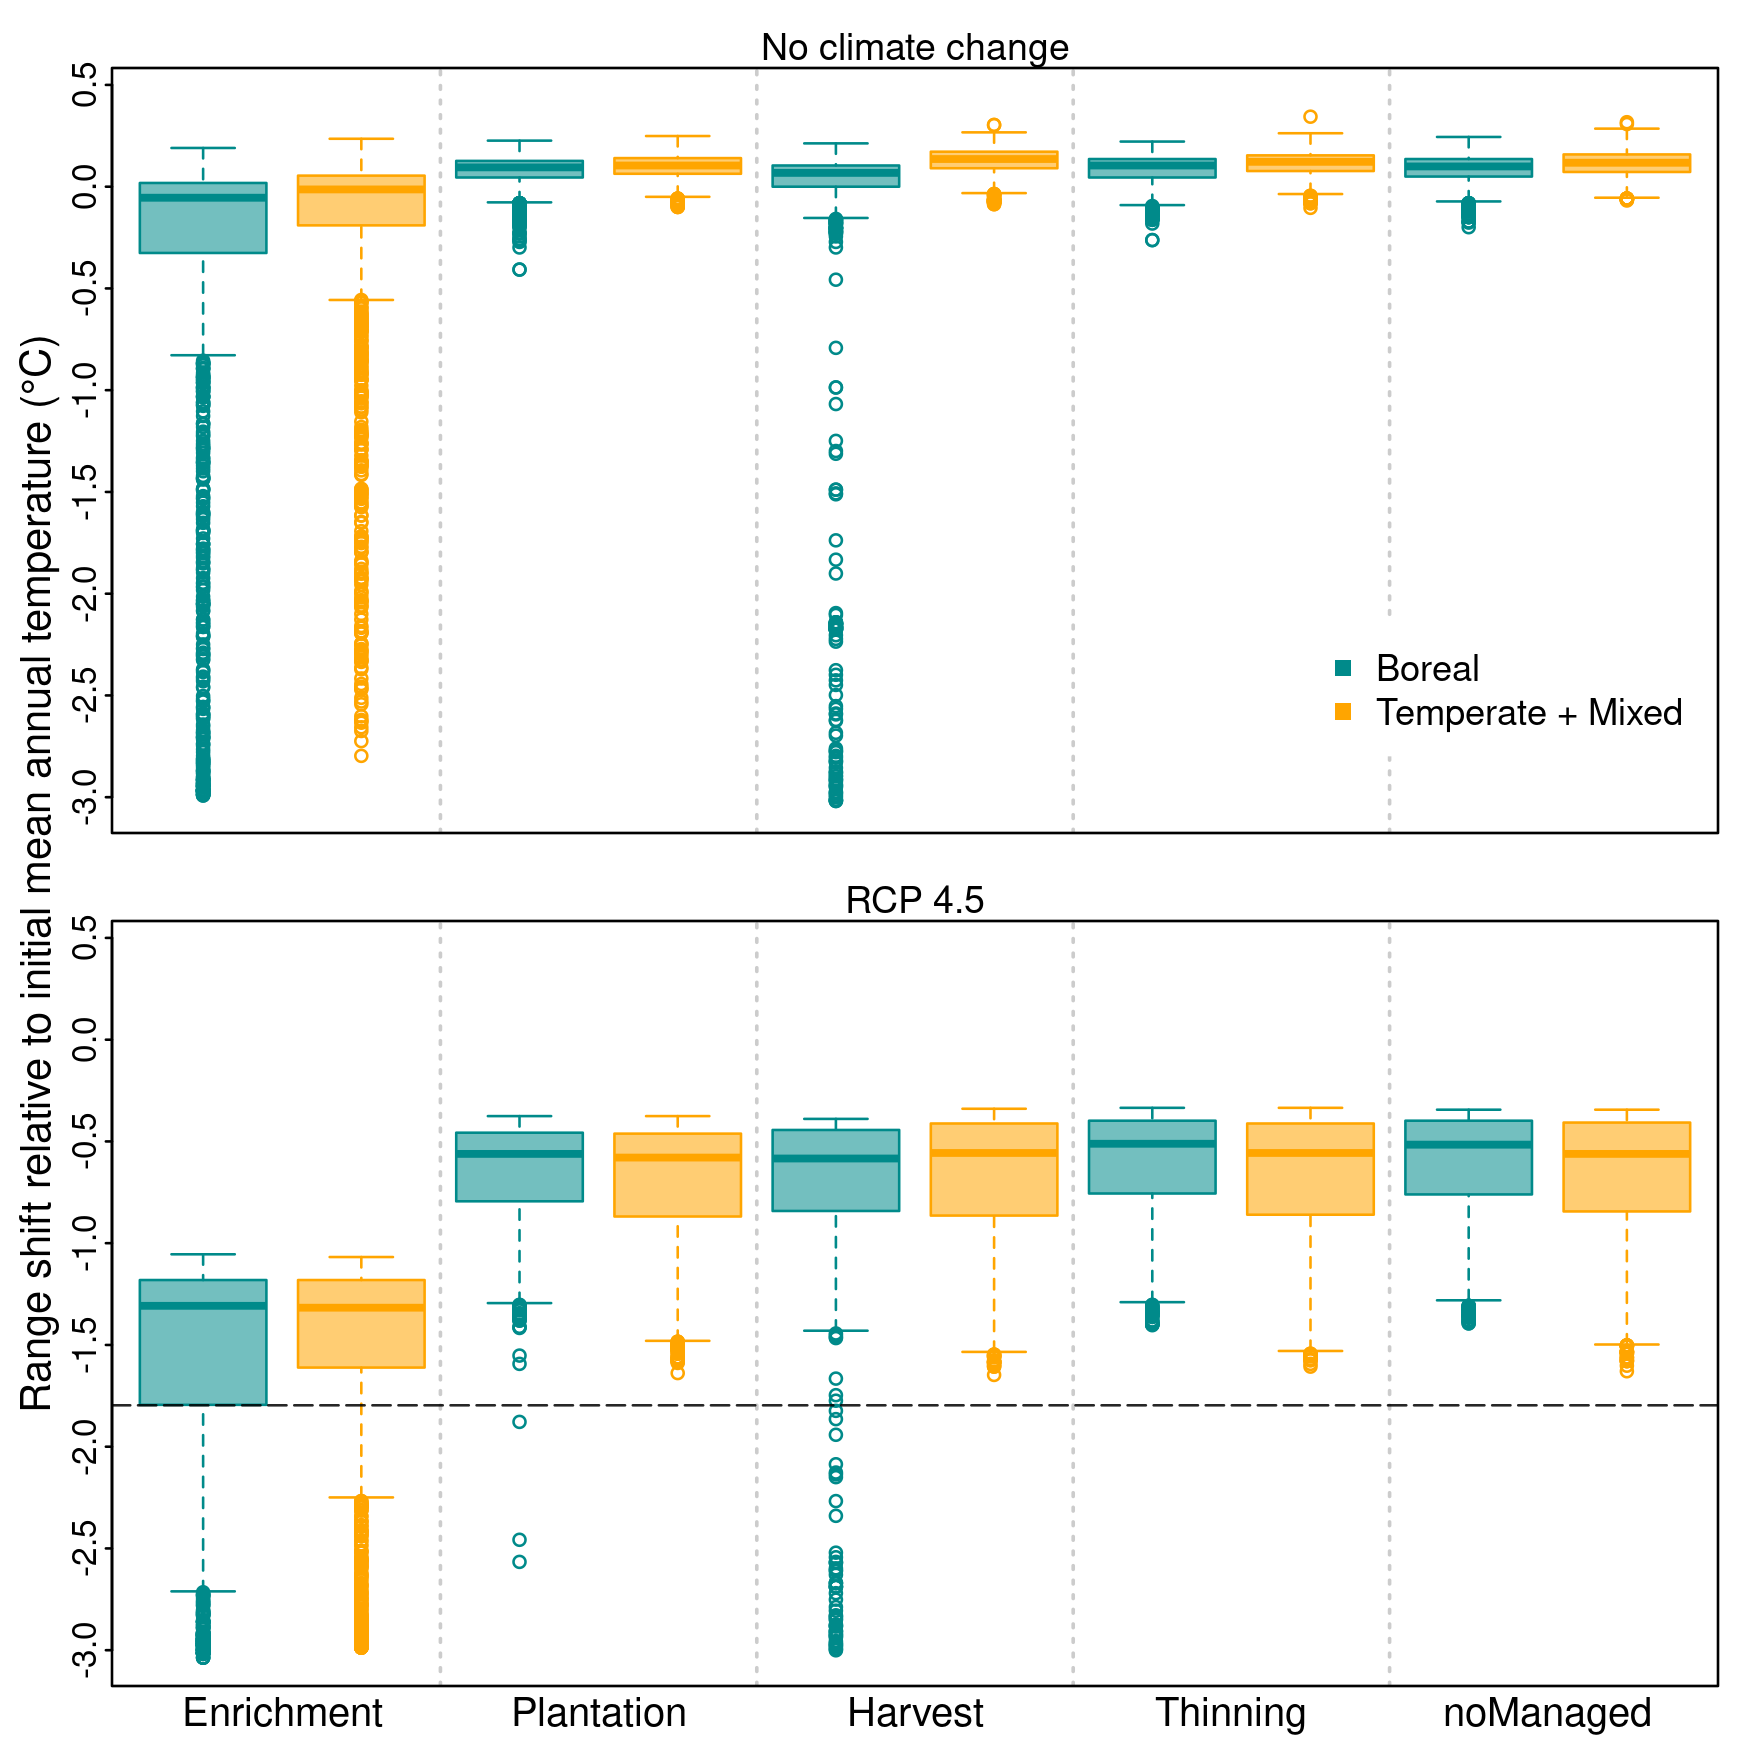
\includegraphics[width=0.75\textwidth,height=\textheight]{manuscript/img/sim-result_3.png}
\caption[{Summary of range shift relative to initial mean annual
temperature for (a) no climate change and (b) climate change under
RCP4.5 scenario.}]{Summary of range shift relative to initial mean
annual temperature for (a) no climate change and (b) climate change
under RCP4.5 scenario. Range shift is the difference between the initial
(\(T_0\) at equilibrium) and final state distribution after 150 years of
simulation. Negative values of range shift indicate a change in forest
distribution towards colder temperature whereas positive values indicate
a change towards warmer temperature. The horizontal dashed line
represents the median expected range shift when model reaches the
equilibrium. Management intensity was set to 0.25\% for plantation,
thinning, and enrichment planting, and 1\% for harvest.}
\label{fig:sim-result2}
\end{figure}
}

Increasing management intensity of up to 20\% per year, while keeping
the simulations running for 150 years, had different effects according
to the four management practices (Figure \ref{fig:sim-result3}; Figure
\ref{fig:sim-result-supp5_ch1}). At an intensity of 5\%, enrichment planting nearly approached the
maximum range shift allowed by the landscape size, with a median range
shift of -3.22 \(^{\circ}\)C, increased to -3.26 and -3.30 \(^{\circ}\)C
for the 10 and 20\% intensity, respectively. Plantation also exceeded
the expected equilibrium at the intensity of 10 and 20\%, with a median
range shift of -2.05 and -3.05 \(^{\circ}\)C, respectively. Harvest was
the only practice to not increase both the boreal and the
temperate-mixed range shift at the same rate. While harvest increased
boreal range shift up to -3.33 \(^{\circ}\)C with 20\% management
intensity, temperate-mixed increased from -0.55 \(^{\circ}\)C (2\%) to
-0.64 \(^{\circ}\)C (20\%). Increasing thinning intensity did not
increase the range shift of the boreal-temperate ecotone towards colder
temperatures, with a stable range shift around -0.53 \(^{\circ}\)C.\\

\hypertarget{fig:sim-result3}{%
\begin{figure}
\centering
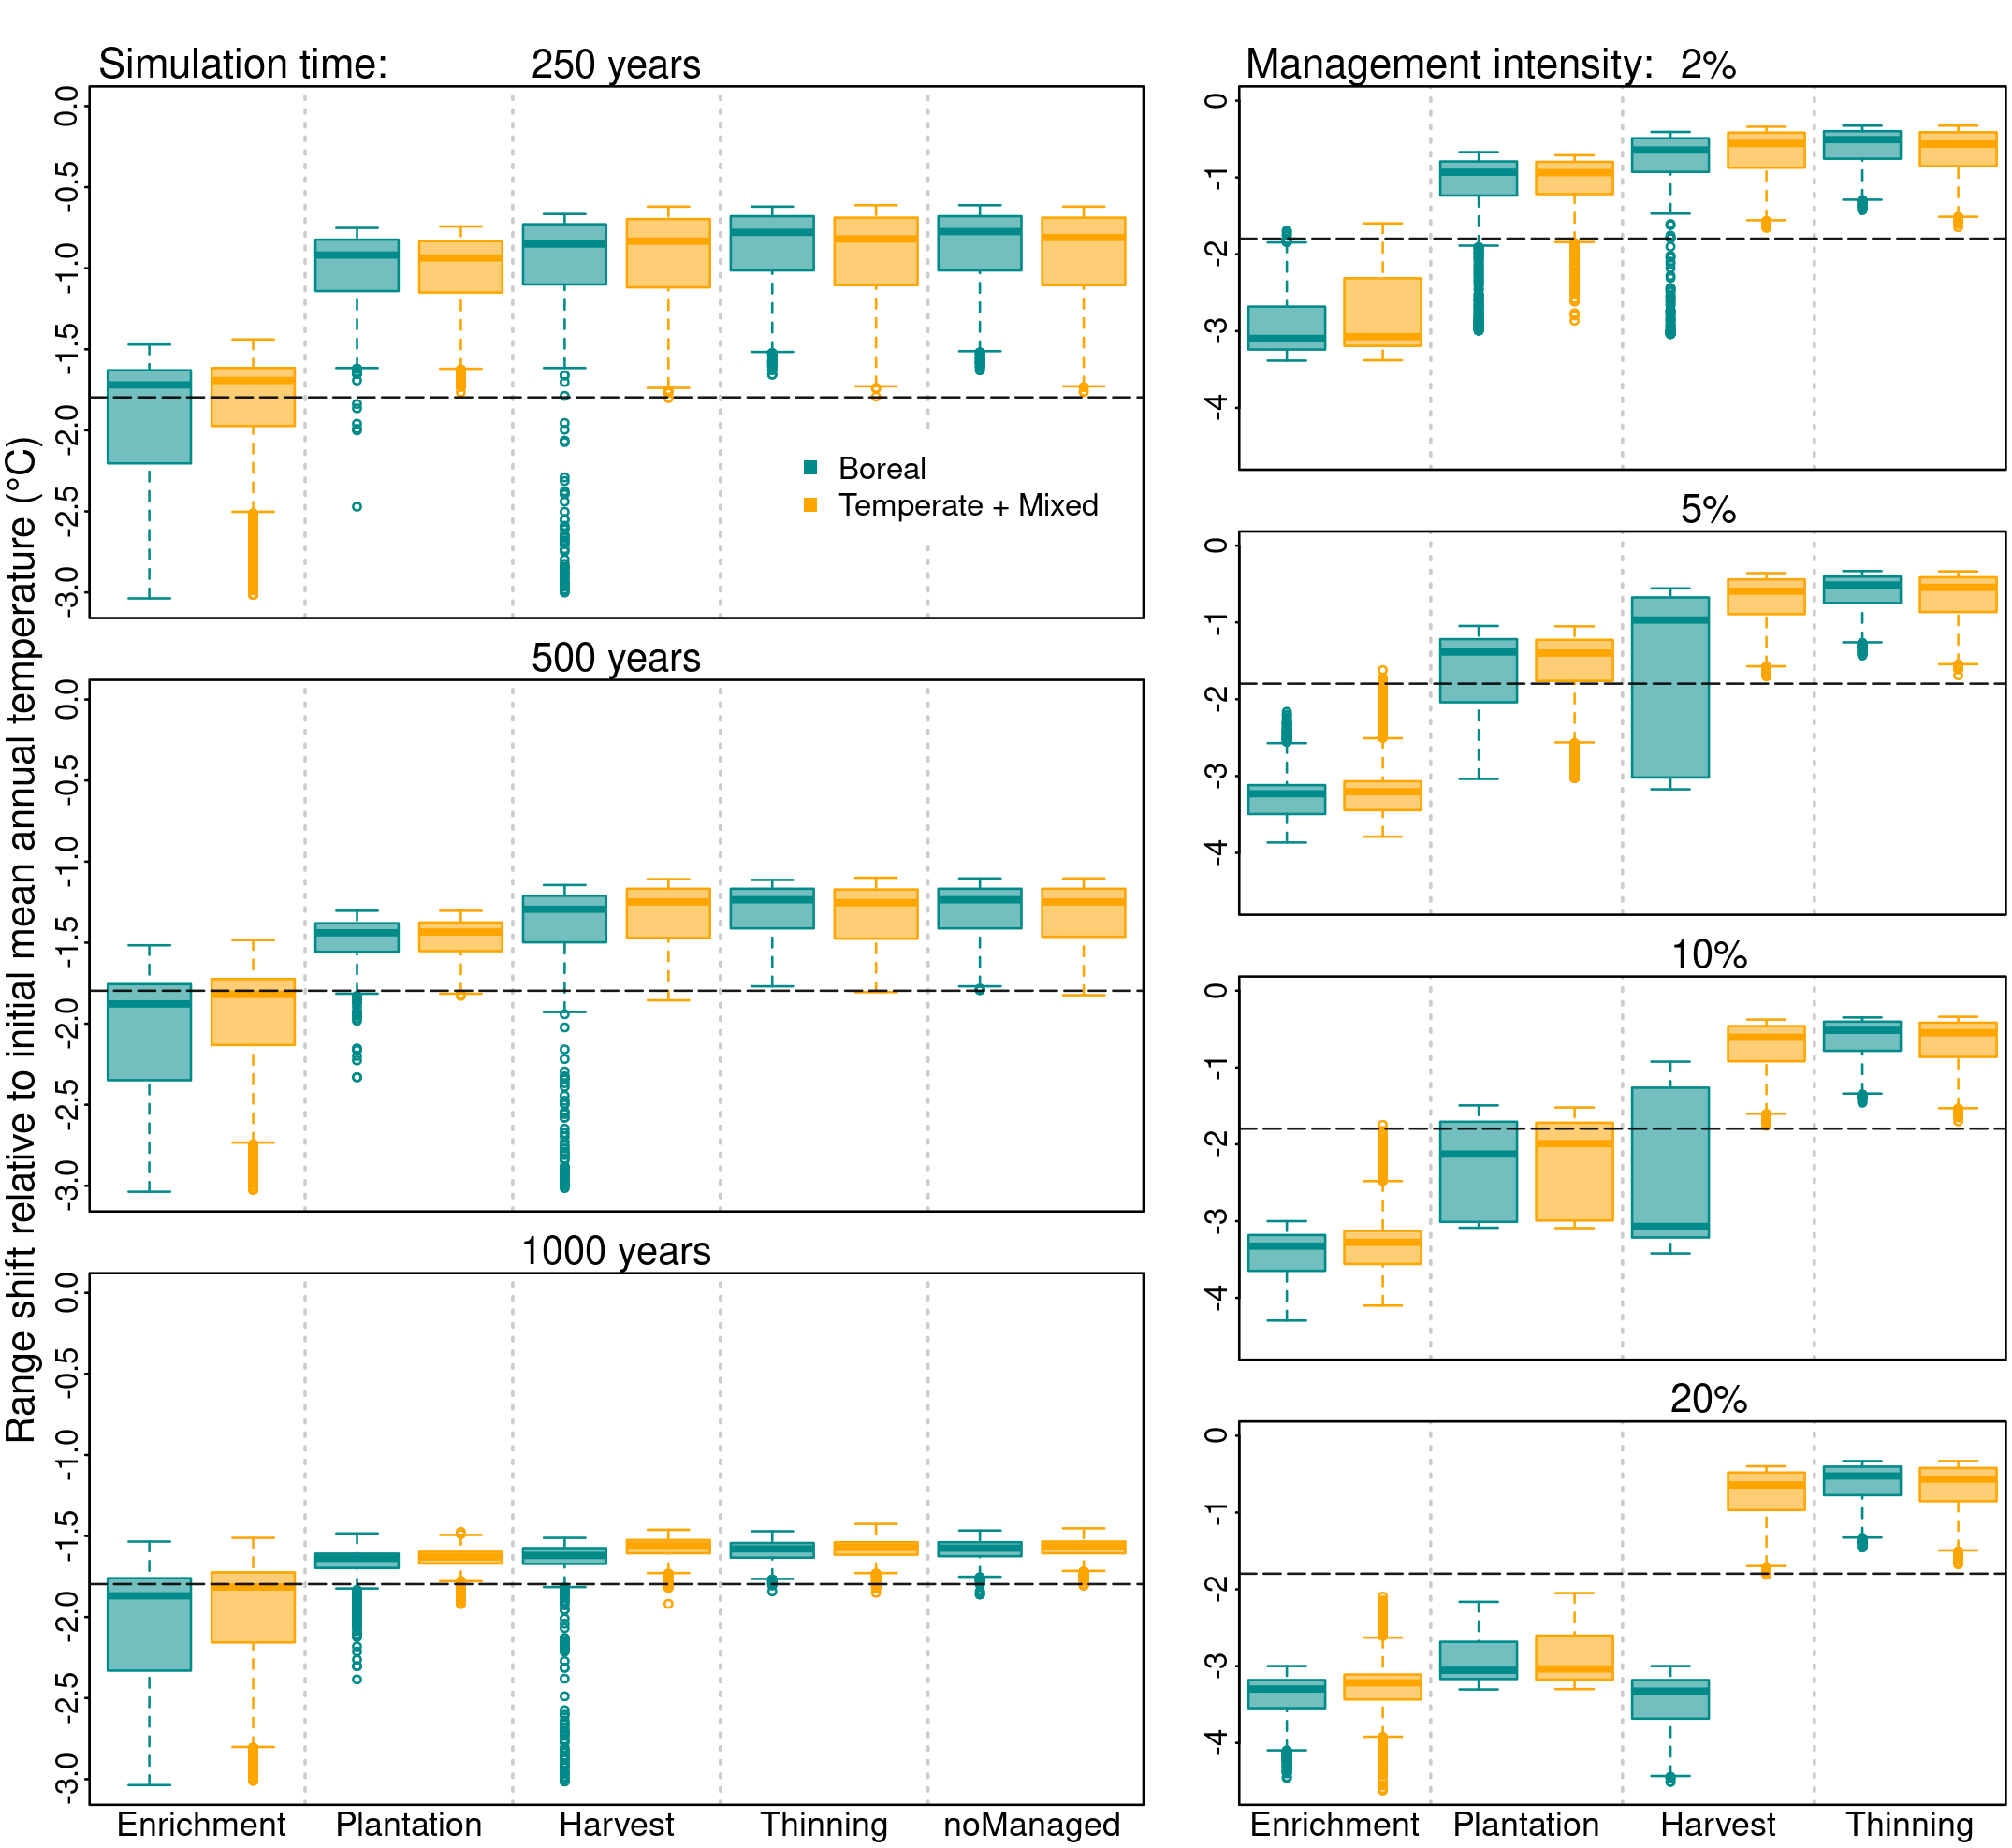
\includegraphics{manuscript/img/sim-result_4.png}
\caption[{Summary of range shift relative to initial mean annual
temperature for different simulation times (a-c) and management
intensities (d-g).}]{Summary of range shift relative to initial mean
annual temperature for different simulation times (a-c) and management
intensities (d-g). Range shift is the difference between the initial
(\(T_0\) at equilibrium) and final state distribution after (i) 150
years of simulation for the panels d-g and (ii) 250, 500, and 1000 years
for the panels a-c.~Negative values of range shift indicate a change
towards colder temperature whereas positive values indicate a change
towards warmer temperature. The horizontal dashed lines represent the
median expected range shift when model reaches the equilibrium for the
particular simulation set. Management intensity was set to 0.25\% for
plantation, thinning, and enrichment planting, and 1\% for harvest for
the panels a-c.~For the panels d-g, management intensity for all the
four practices was set to 2, 5, 10, or 20\%, respectively.}
\label{fig:sim-result3}
\end{figure}
}

\hypertarget{discussion}{%
\section{Discussion}\label{discussion}}

It is pressing to investigate how forest biomes will respond to climate
warming, and how forest management can mitigate the negative impacts of
this perturbation. We extended a simple and informative modelling
framework based on metapopulation theory that let us to (i) establish a
link between forest management and the ecological processes setting
range limits, and (ii) investigate the effect of forest management on
the response of the boreal-temperate ecotone to climate change. Our
study suggests, based on two complementary simulation techniques, that
forest management could help the boreal-temperate ecotone keep pace with
climate change. Paying colonization credit by enrichment planting of
temperate tree species in boreal forest stands, and the plantation of
temperate species in regenerating stands, are likely to increase forest
resilience, reduce the time to reach a new equilibrium, and increase
range limit shifts towards colder temperatures. This theoretical
investigation provides new opportunities to design future experiments
testing the potential of forest management to adapt to climate change.
It should guide forest managers to take into account both natural and
anthropogenic disturbances on forest dynamics.\\

\textbf{\emph{How can plantation and enrichment planting reduce
colonization credit?}}

Although climate change is expected to drive a shift in forest
composition by favoring temperate over boreal trees, the
boreal-temperate ecotone is lagging behind climate change
\citep{BoisvertMarsh2014, BoisvertMarsh2019, Talluto2017, Vissault2020}.
Similar results are found on altitudinal gradients, where the slow
dieback of \emph{Picea abies} prevents the expansion of other species
\citep{Scherrer2020}. Our results suggest that plantation and enrichment
planting of temperate species on the boreal region can increase the
response of the boreal-temperate ecotone to climate warming by reducing
the transient period and increasing the range shift towards colder
temperatures. To date, few studies have tested how assisted migration
can shift trees' range limits. For instance, modelling the plantation of
tree species more suitable to future climate is predicted to increase
resilience indicators such as carbon stocks and tree species diversity
\citep{Hof2017}, and therefore plantation is assumed to increase tree
range shift under climate change. Using the same rationale, simulating
the plantation of tree species in future suitable enviroments was
demonstrated to increase both biomass productivity and species diversity
in multiple scenarios of climate change \citep{Duveneck2015}. We found
that enrichment planting slightly increased asymptotic resilience, which
indicates a faster recovery to equilibrium after climate change (Figure
\ref{fig:num-res1}). This is similar to a modelling study that suggests
forest management had limited ability to increase resistance and
resilience under climate change \citep{Duveneck2016}.\\

\textbf{\emph{Why is enrichment planting practice more efficient than
planting?}}

Enrichment planting of temperate trees into boreal areas had a stronger
effect on both reducing the transient period and increasing range shift
when compared with planting temperate in disturbed (empty) areas. This
is due to three different mechanisms. First, the intensity of forest
management in the model is relative to the abundance of a particular
forest type in the lanscape (Figure \ref{fig:sim-result-sup8_ch1}); hence 0.25\% of boreal stands
being enriched is much higher than 0.25\% of regeneration stands being
planted since the number of boreal stands is proportionally larger than
the number of regeneration stands. That explains the need to increase
planting intensity beyond 0.25\% to increase the boreal range shift
towards colder temperatures (Figure \ref{fig:sim-result-supp5_ch1}). Second, management practices
are not spatially organized. While enrichment planting is necessarily
applied on boreal stands (and thus in the colonization credit area),
planting is applied in regeneration stands that are evenly distributed
across the landscape, including the mixedwood and temperate regions.
Finally, while enrichment planting implies both an increase of temperate
trees and a reduction of boreal stands, plantation involves only an
increase of temperate stands. These results suggest that enrichment
planting in local gaps has the best potential compared to plantation to
assist forests keep pace with climate change. For northern temperate
forests with different levels of shade tolerance, tree recruitment was
more effective in the presence of local canopy gaps compared to
recruitment in open areas after clearcut \citep{LePage2000}.\\

\textbf{\emph{Why does reducing colonization credit increase range shift
but reducing extinction debt does not?}}

Reducing extinction debt by increasing the frequency of disturbance
(natural or anthropogenic) is expected to drive range shift by
eliminating maladapted species that would persist for a long period, and
then create colonization opportunities for advancing species
\citep{Renwick2015, Kuparinen2010}. Here intensifying disturbance by
increasing harvest of boreal stands did not affect the rate of range
shift after temperature increases. This result corroborates with those
of \citet{Vanderwel2014} who found that harvesting boreal species
amplifies transitions to early-successional forest type, but has no
effect on the range shift of boreal conifers. Similarly expect for the
disturbance intensity, \citet{Brice2020} also found that moderate
disturbances increased the probability of transition from mixedwood to
temperate stands but had a small effect on the transition from boreal to
mixedwood. Such a lack of effect on range shift may be explained by the
fact that most harvested boreal stands regenerate to boreal again due to
source-sink dynamics and the ecosystem internal memory such as seed
bank. In a field experiment, \citet{Reich2015} showed that the growth
rate of juvenile trees increased in their colder range and decreased in
their warmer range when exposed to above and belowground temperature
increases. In other words, temperate trees will perform better than
boreal trees in the transition between their ranges. Therefore, limited
dispersal rather than competition may be the primary factor contributing
for a lack of temperate colonization in harvested patches.\\

\textbf{\emph{Thinning increases temperate tree range expansion, but
does not affect boreal stands}}

We explored the hypothesis that selective harvesting of boreal tree
species (thinning) on stands in state M would increase the proportion of
stands in state T in the landscape, and therefore increase the regional
pool to favor the colonization of temperate trees into the boreal
region. Thinning indeed increased the proportion of temperate stands in
the mixedwood region by an increase in competitive exclusion
(\(\theta_{m}\) and \(\theta_{T, m}\)). Similar results have been shown
that harvest increased temperate species in the mixedwood region of
Quebec \citep{Boulanger2019, Brice2020}. However, our model also show
that thinning did not have any effect on the range limit of boreal
stands. In other words, temperate trees did not colonize boreal stands,
even with a increasing source pools. Such a lack of temperate
progression onto the boreal region may be explained by the difficulty of
temperate trees to settle in boreal stands due to priority effects and
unfavourable substrates \citep{Solarik2018, Solarik2020}. This effect is
included in the model indirectly through the invasion (mean
\(\beta_{T}\) = 0.62) and colonization (mean \(\alpha_{T}\) = 0.99)
parameters associated with the temperate stand. This may be the result
of plant-soil feedbacks or the importance of gaps for temperate tree
regeneration. For instance, regeneration of temperate species such as
red maple and red oak has been shown to be facilitated in forest gaps,
while most boreal species showed no difference \citep{Leithead2010}.\\

\textbf{\emph{Limitations and future perspectives}}

We have found that plantation and enrichment planting have the potential
to reduce colonization credit to help forests to keep pace with climate
change. However, further experiments are necessary as the four simulated
practices in our study are an approximation of real management
practices. For instance, we simulated thinning as selective logging
boreal species in favor of temperate species, while in practice,
thinning generally focuses on reducing stand density and maintaining
commercial species. Such density reduction is tricky to address with our
model because local abundances are not accounted for. There is generally
a mismatch between our simulations at the community stand resolution
with the management practices that occur from the individual to the
population level. Being aware of that caveat, we urge future modelling
studies to concomitantly represent forest dynamics at several
organizational levels, while including detailed management practices.
Individual-level models accounting for demographic rates are useful to
predict how local mechanisms such as species interaction can scale up to
determining species range limits
\citep{Araujo2014a, Normand2014, Snell2014}. Moreover, forest-landscape
models and dynamic vegetation models can more accurately simulate the
migration process \citep{Lehsten2019}. In our context, individual-level
models can test the effect of forest management on growth, mortality,
and regeneration, while a community-level model such as ours helps
better understand how the effect of management practices scales up. We
should also cautiously interpret the effect of climate change as
simulated here. Although it is predicted that drought intensity will
increase in the future and may drive how the forest will respond to
climate change \citep{Greenwood2017}, we have simulated only temperature
warming, while precipitation remained constant. Some studies have shown
tree species to be more sensitive to an increase in drought rather than
temperature \citep[\emph{e.g.} white spruce][]{Andalo2005}. Drought is,
however, more a pulse disturbance (or shock), having potential
cumulative effects on trees, and involving thresholds. Moreover, it
should be investigated with various frequencies and intensities. The
present study rather shows how forest management could help communities
adapt to a continuous change in the environment, mainly driven by
changes in temperature.\\

We have provided evidence that management practices could help forest
communities cope with the rate at which climate change is occurring
across the southern half of Quebec. However, we can expect the final
outcome to be sensitive to the spatial distribution of different
practices. For instance, harvesting boreal stands nearby the leading
edge of the mixedwood distribution may create a synergy. On the other
hand, a 20\% harvest intensity had a strong effect on the range shift of
boreal forest, while the temperate range did not move (Figure
\ref{fig:sim-result3} g), showing that there are other factors more
important than the spatial distribution of the management practice. We
have simulated here the effect of four management practices alone in
order to distinguish the most effective and identify the potential
important mechanisms. However, the interaction between management
practices may have synergic or cancelling effects. Our simulations show
no effect of plantation and harvest on the range shift of the
boreal-temperate ecotone at a short time scale of 150 years (figure
\ref{fig:sim-result}). However, planting temperate trees after
harvesting boreal stands may overcome the limitations of these two
practices when applied individually, specially if these practices are
applied in particular locations such as in the transition zone. We
propose future studies should focus on integrating different spatial and
organizational forest models \citep[e.g.~][]{talluto2016}, so that the
link between a management practice and the ecological processes can be
better adjusted and detailed according to its specific scale.\\

\singlespacing
{\renewcommand{\bibname}{References}
\renewcommand{\bibsection}{\section{\bibname}}
\bibliography{chapter1/manuscript/references}}
\bibliographystyle{styles/myBEAS}
